\section{Слежение и компенсация: матричные уравнения}

\subsection{Анализ системы}

Рассмотрим систему
\begin{equation}
    \label{eq:sys1}
    \begin{cases}
        \dot x=Ax+Bu+B_ff,\\
        y=Cx+Du+D_ff,
    \end{cases}\quad
    x(0)=\begin{bmatrix}
        0&0&0
    \end{bmatrix}^T,
\end{equation}
где
\begin{equation*}
    A=\begin{bmatrix}
        3&5&4\\-2&-4&-5\\2&2&3
    \end{bmatrix},\quad
    B=\begin{bmatrix}
        2\\-1\\1
    \end{bmatrix},\quad
    B_f=\begin{bmatrix}
        -2&2\\-2&0\\0&0
    \end{bmatrix},\quad
    C=\begin{bmatrix}
        -2\\-1\\0
    \end{bmatrix}^T,\quad
    D=\begin{bmatrix}
        1
    \end{bmatrix},\quad
    D_f=\begin{bmatrix}
        4\\1
    \end{bmatrix}^T,
\end{equation*}
генератор внешнего возмущения
\begin{equation}
    \label{eq:sys1gen}
    \begin{cases}
        \dot w_f=\Gamma_fw_f,\\
        f=Y_fw_f,
    \end{cases}\quad
    w_f(0)=\begin{bmatrix}
        1&1&1&1
    \end{bmatrix}^T,
\end{equation}
где
\begin{equation*}
    \Gamma_f=\begin{bmatrix}
        35 &56& 22& -42\\
        -11& -17 &-7 &12\\
        -6 &-10& -5& 10\\
        11 &18 &6 &-13
    \end{bmatrix},\quad
    Y_f=\begin{bmatrix}
        1 &3\\
        2& 4\\
        1 &2\\
        -1 &-3
    \end{bmatrix},
\end{equation*}
и генератор  задающего воздействия
\begin{equation}
    \label{eq:sys1g}
    \begin{cases}
        \dot w_g=\Gamma_gw_g,\\
        g=Y_gw_g,
    \end{cases},\quad
    w_g(0),
\end{equation}
где $g(t)=8\cos(5t)+2,$ тогда
\begin{equation*}
    \Gamma_g=\begin{bmatrix}
        0 & 5 & 0 \\
        -5& 0 & 0 \\
        0 & 0 & 0
    \end{bmatrix},\quad
    Y_g=\begin{bmatrix}
        8 & 0 & 2
    \end{bmatrix},\quad
    w_g(0)=\begin{bmatrix}
        1 & 0 & 1
    \end{bmatrix}.
\end{equation*}
Собственные числа матрицы $\Gamma_f$ следующие
\begin{equation}
    \label{eq:specGf}
    \sigma(\Gamma_f)=\{\pm3i,\ \pm i\},
\end{equation}
внешнее возмущение имеет вид суммы гармоник:
\begin{equation*}
    w_{f_i}(t)=a_i\cos(t)+b_i\sin(t) + c_i\cos(3t)+d_i\sin(3t).
\end{equation*}
Собственные числа матрицы $\Gamma_g$ следующие
\begin{equation}
    \label{eq:specGg}
    \sigma(\Gamma_g)=\{\pm5i,\ 0\}.
\end{equation}
\begin{figure}[H]
    \centering
    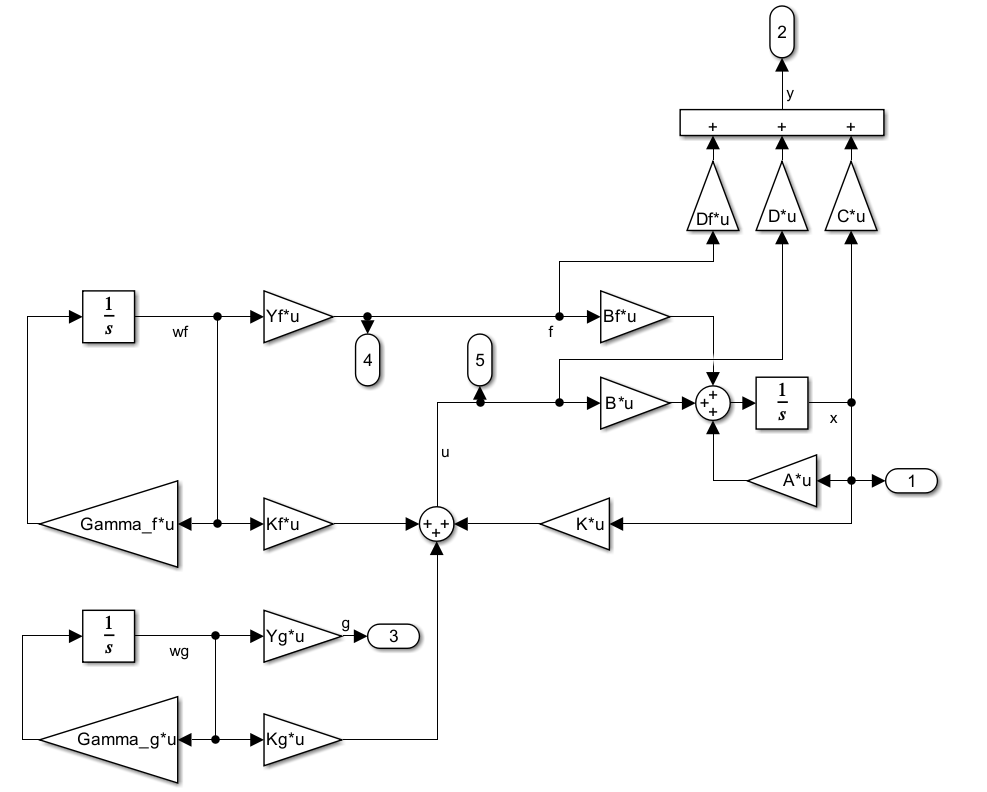
\includegraphics[width=\linewidth]{figs/10slx.png}
    \caption{Схема моделирования системы \eqref{eq:sys1}}
    \label{fig:sys1}
\end{figure}
Построить схему (\autoref{fig:sys1}) моделирования системы \eqref{eq:sys1}, 
замкнутой регулятором
\begin{equation}
    \label{eq:reg1}
    u=Kx+K_gw_g+K_fw_f,
\end{equation}
обеспечивающим выполнение целевого условия
\begin{equation}
    \label{eq:goal1}
    \lim_{t\rightarrow\infty}|g(t)-y(t)|=0.
\end{equation}

\subsection{Синтез регулятора}

\subsubsection{Синтез «feedback»-компоненты}

Синтезировать «feedback»-компоненту как LQR.
Зададимся значениями матриц $Q\succ0$ и $R\succ0$:
\begin{equation*}
    Q=\begin{bmatrix}
        1 & 0 & 0\\
        0 & 1 & 0\\
        0 & 0 & 1
    \end{bmatrix},
    R=1,
\end{equation*}
и решим соответствующее уравнение Риккати:
\begin{equation}
    \label{eq:ric1}
    A^TP+PA-PBR^{-1}B^TP+Q=0,\quad K=-R^{-1}B^TP.
\end{equation}
С помощью функции \texttt{icare} в MATLAB получили:
\begin{equation}
    \label{eq:K}
    K =\begin{bmatrix}
        -1.5798&	-1.3778	&-7.1171
    \end{bmatrix}.
\end{equation}

\subsubsection{Синтез «feedforward»-компоненты для слежения}

Система матричных уравнений Франкиса-Дэвисона для синтеза 
следящей компоненты $K_g$ регулятора \eqref{eq:reg1} следующая:
\begin{equation*}
    \begin{cases}
        P_g\Gamma_g-(A+BK)P_g=BK_g\\
        (C+DK)P_g+DK_g=Y_g,
    \end{cases}
\end{equation*}
для существования решения необходимо проверить ранги следующих матриц:
\begin{gather*}
    rank\begin{bmatrix}
        A+BK-5iI & B \\
        C+DK & D
    \end{bmatrix}=4,\quad
    rank\begin{bmatrix}
        A+BK+5iI & B \\
        C+DK & D
    \end{bmatrix}=4,\quad
    rank\begin{bmatrix}
        A+BK & B \\
        C+DK & D
    \end{bmatrix}=4.
\end{gather*}
Все ранги равны 4, значит, система имеет решение.
С помощью CVX в MATLAB получили:
\begin{equation}
    \label{eq:Kg}
    K_g=\begin{bmatrix}
        0.2677	&-1.1433	&0.5000
    \end{bmatrix}.
\end{equation}

\subsubsection{Синтез «feedforward»-компоненты для компенсации}

Система матричных уравнений Франкиса-Дэвисона для синтеза 
компенсирующей компоненты $K_f$ регулятора \eqref{eq:reg1} следующая:
\begin{equation*}
    \begin{cases}
        P_f\Gamma_f-(A+BK)P_f-B_fY_f=BK_f\\
        (C+DK)P_f+DK_gf=-D_fY_f,
    \end{cases}
\end{equation*}
для существования решения необходимо проверить ранги следующих матриц:
\begin{gather*}
    rank\begin{bmatrix}
        A+BK-3iI & B \\
        C+DK & D
    \end{bmatrix}=4,\quad
    rank\begin{bmatrix}
        A+BK+3iI & B \\
        C+DK & D
    \end{bmatrix}=4,\\
    rank\begin{bmatrix}
        A+BK-iI & B \\
        C+DK & D
    \end{bmatrix}=4,\quad
    rank\begin{bmatrix}
        A+BK+iI & B \\
        C+DK & D
    \end{bmatrix}=4.
\end{gather*}
Все ранги равны 4, значит, система имеет решение.
С помощью CVX в MATLAB получили:
\begin{equation}
    \label{eq:Kf}
    K_f=\begin{bmatrix}
        38.5358	&57.3857	&26.7383&	-48.4226
    \end{bmatrix}.
\end{equation}

\subsection{Компьютерное моделирование}

Выполним моделирование разомкнутой системы \eqref{eq:sys1}, результат можно
увидеть на \autoref{fig:10sim}.
Выполним моделирование, замкнутой только «feedback»-компонентой, системы \eqref{eq:sys1}, результат можно
увидеть на \autoref{fig:11sim}.
Выполним моделирование,  замкнутой регулятором без следящей компоненты, системы \eqref{eq:sys1}, результат можно
увидеть на \autoref{fig:12sim}.
Выполним моделирование,  замкнутой регулятором без компенсирующей компоненты, системы \eqref{eq:sys1}, результат можно
увидеть на \autoref{fig:13sim}.
Выполним моделирование системы \eqref{eq:sys1} замкнутой регулятором \eqref{eq:reg1}, результат можно
увидеть на \autoref{fig:14sim}.

\begin{figure}[H]
    \centering
    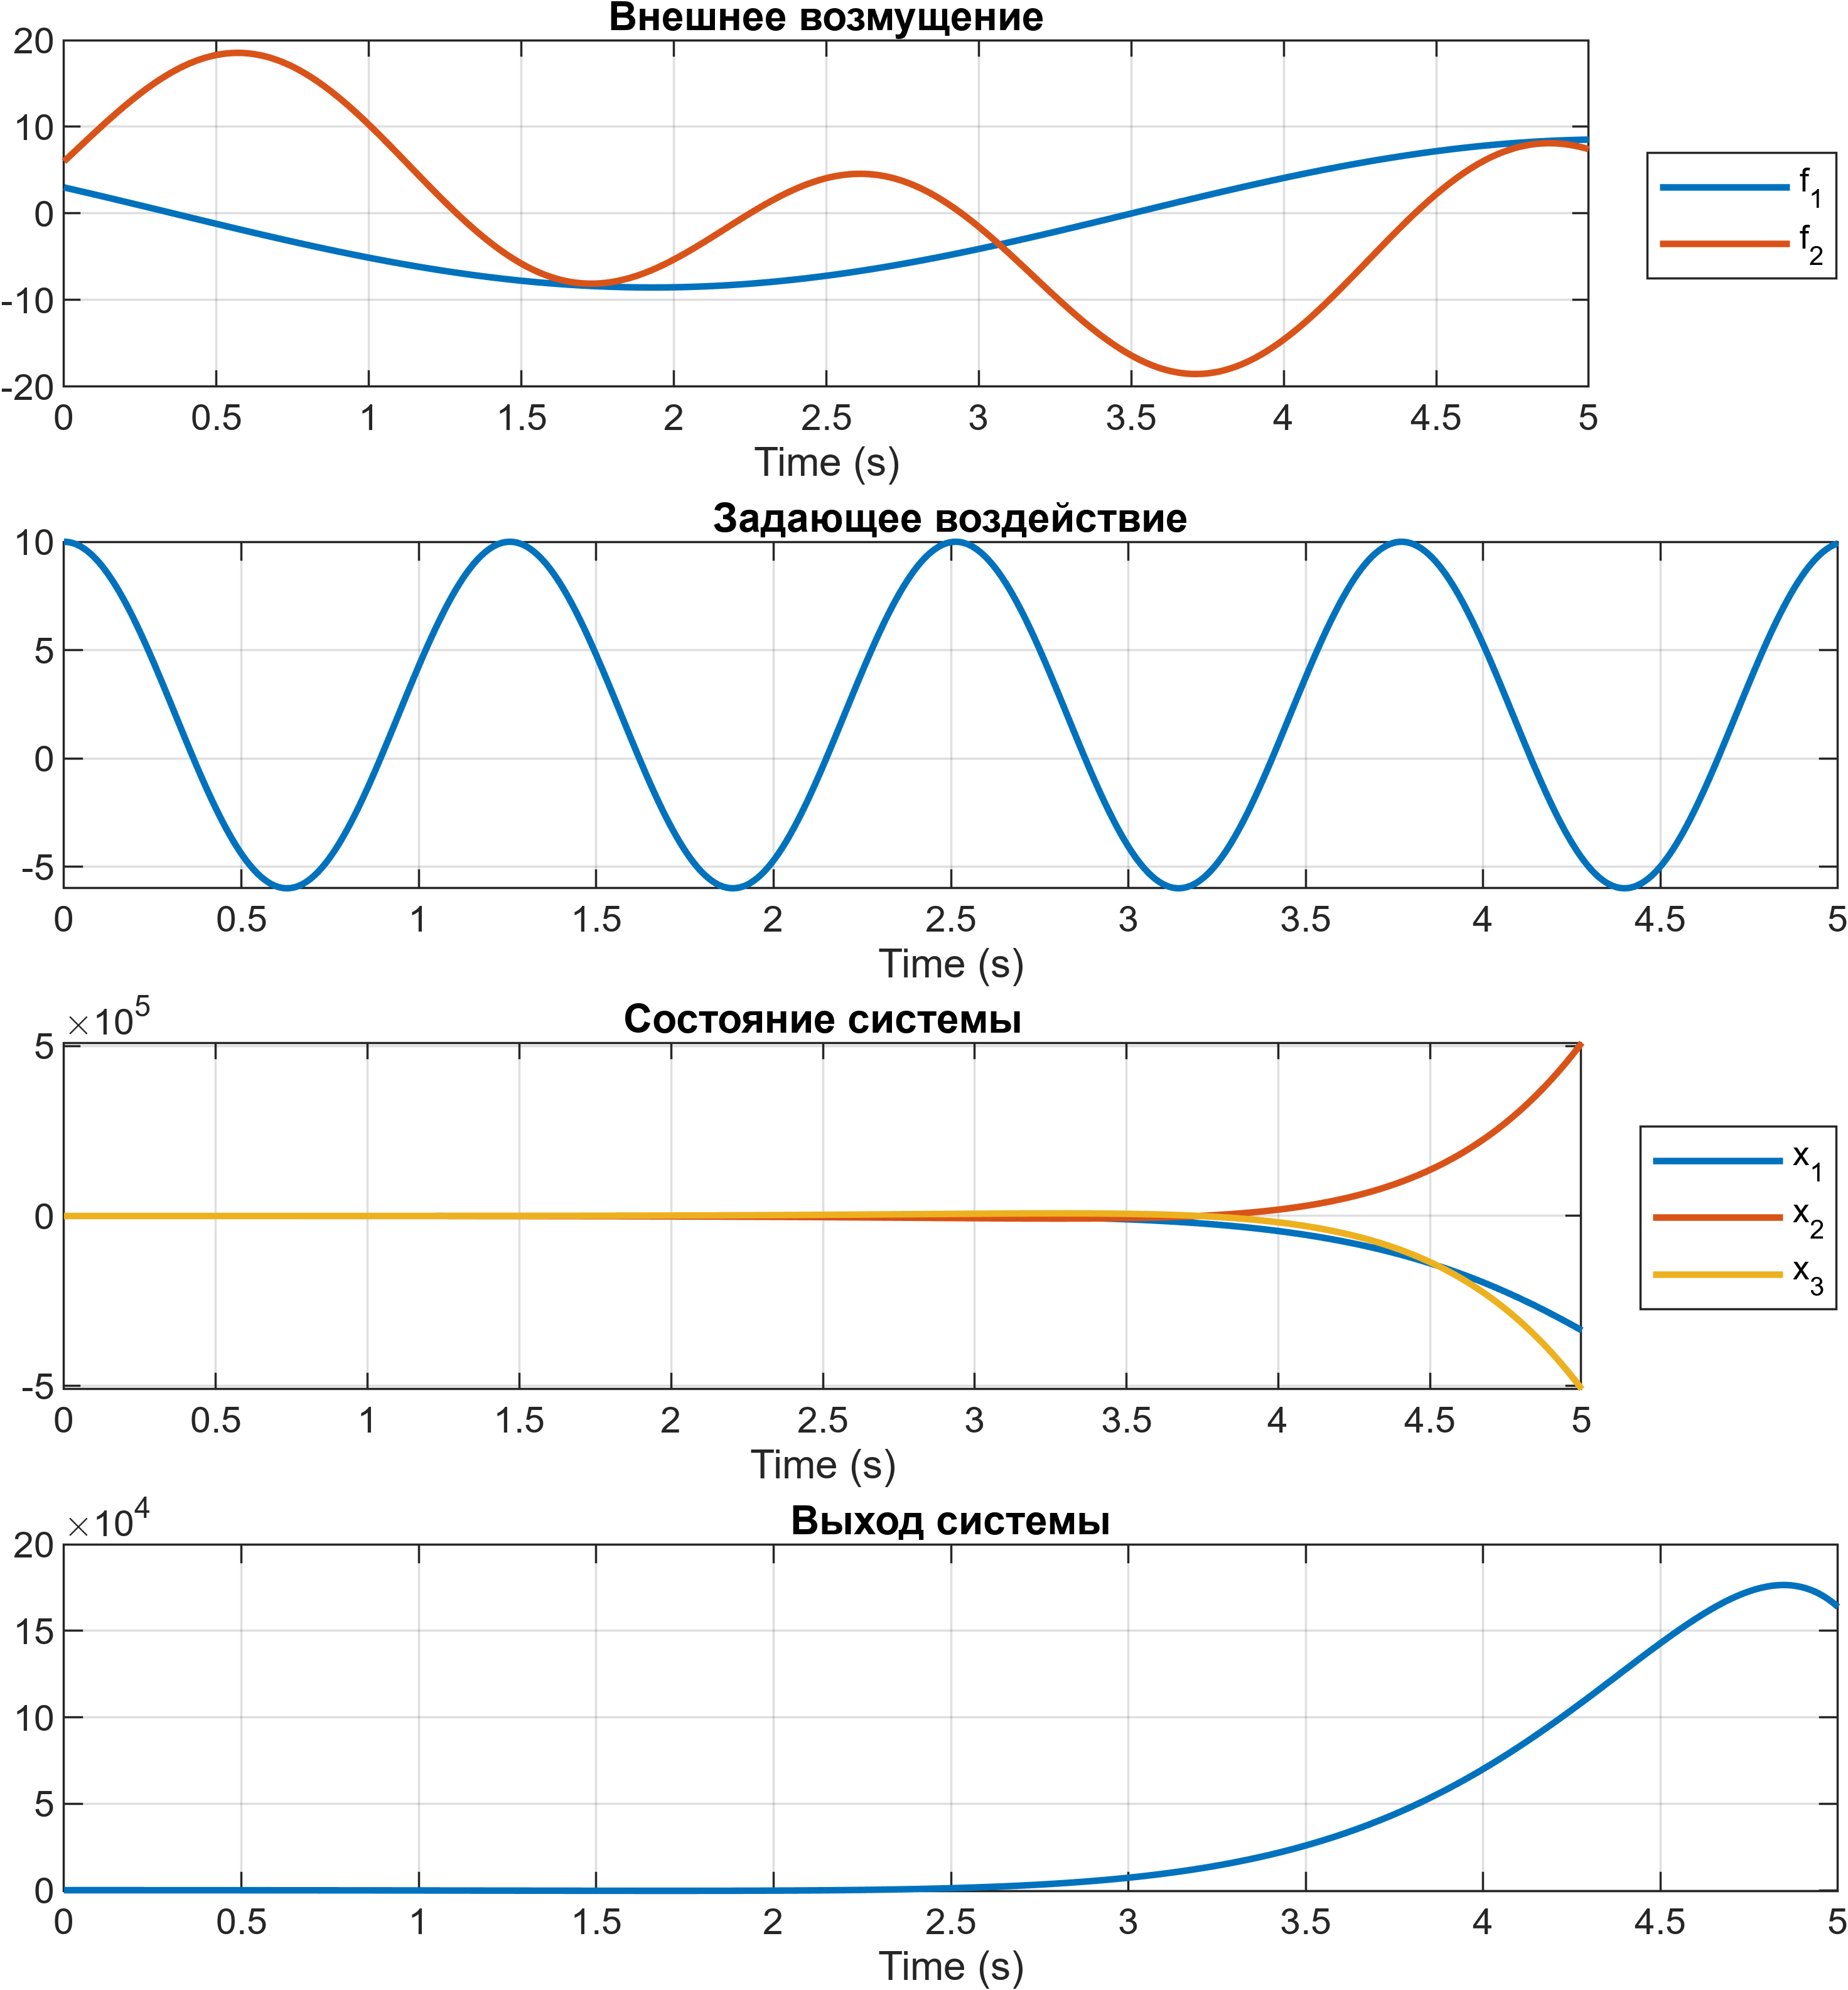
\includegraphics[width=\linewidth]{figs/10_sim.png}
    \caption{Разомкнутая система \eqref{eq:sys1}}
    \label{fig:10sim}
\end{figure}
\begin{figure}[H]
    \centering
    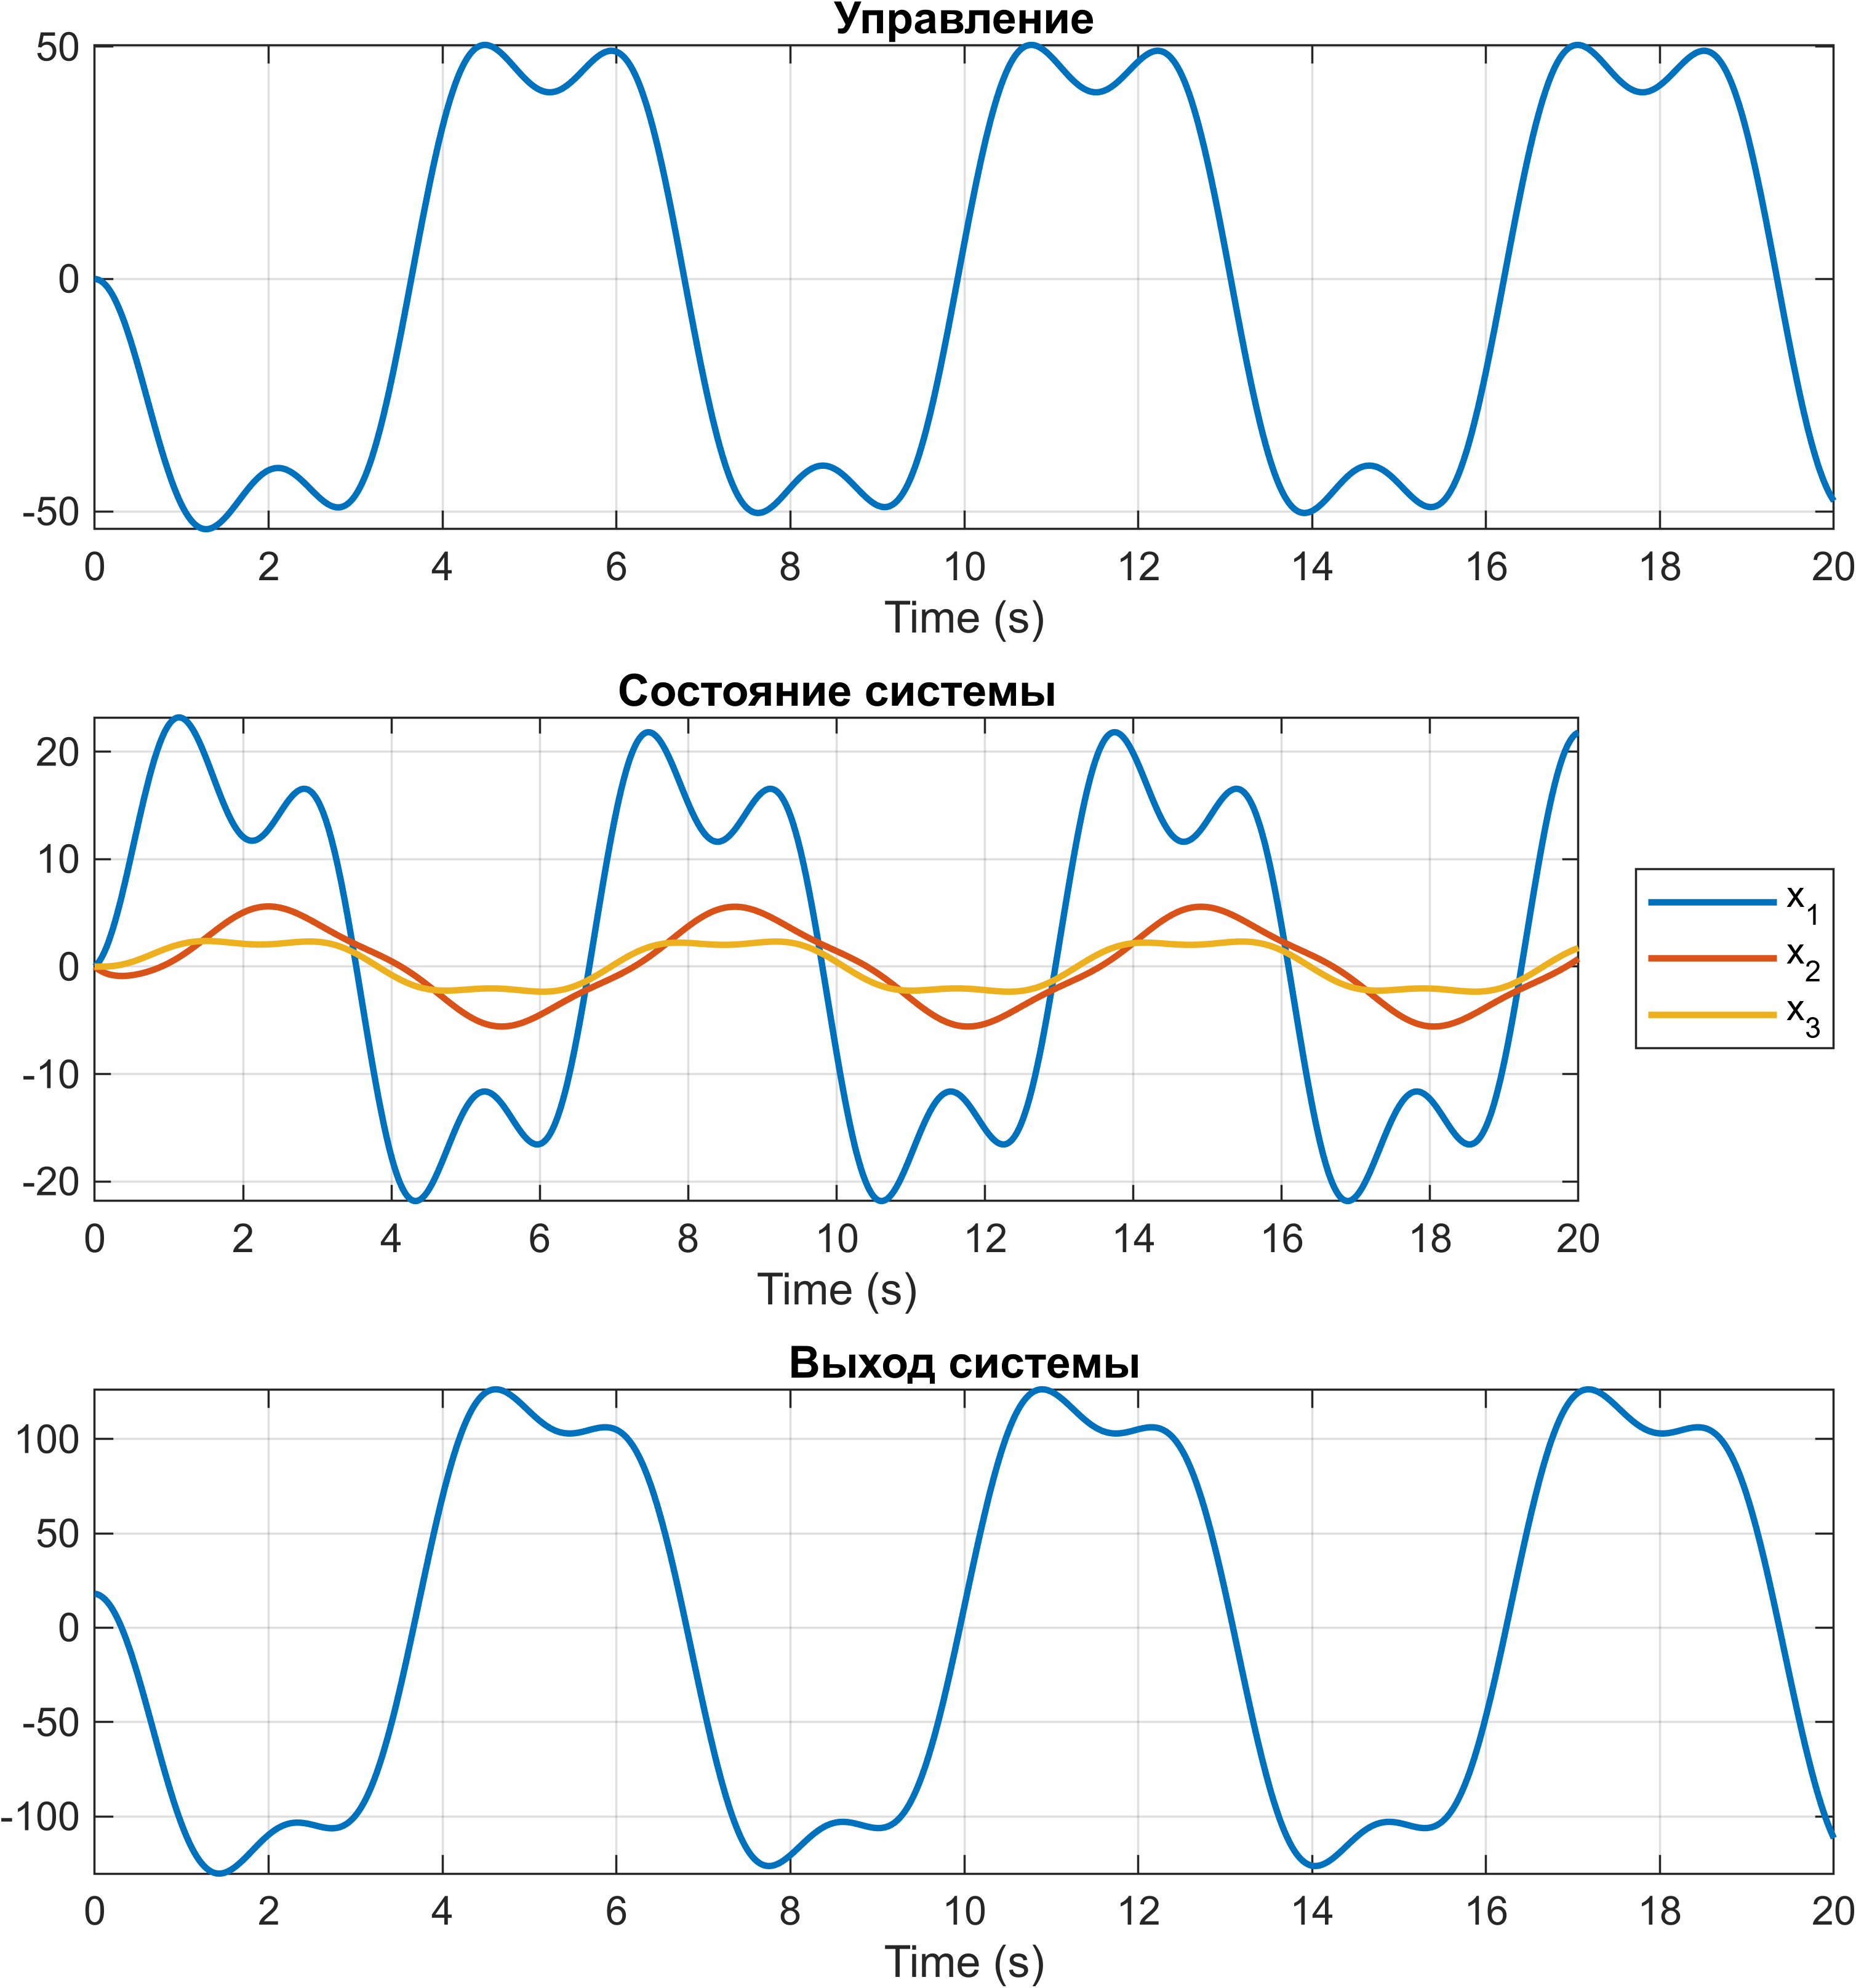
\includegraphics[width=\linewidth]{figs/11_sim.png}
    \caption{Замкнутая только «feedback»-компонентой система \eqref{eq:sys1}}
    \label{fig:11sim}
\end{figure}
\begin{figure}[H]
    \centering
    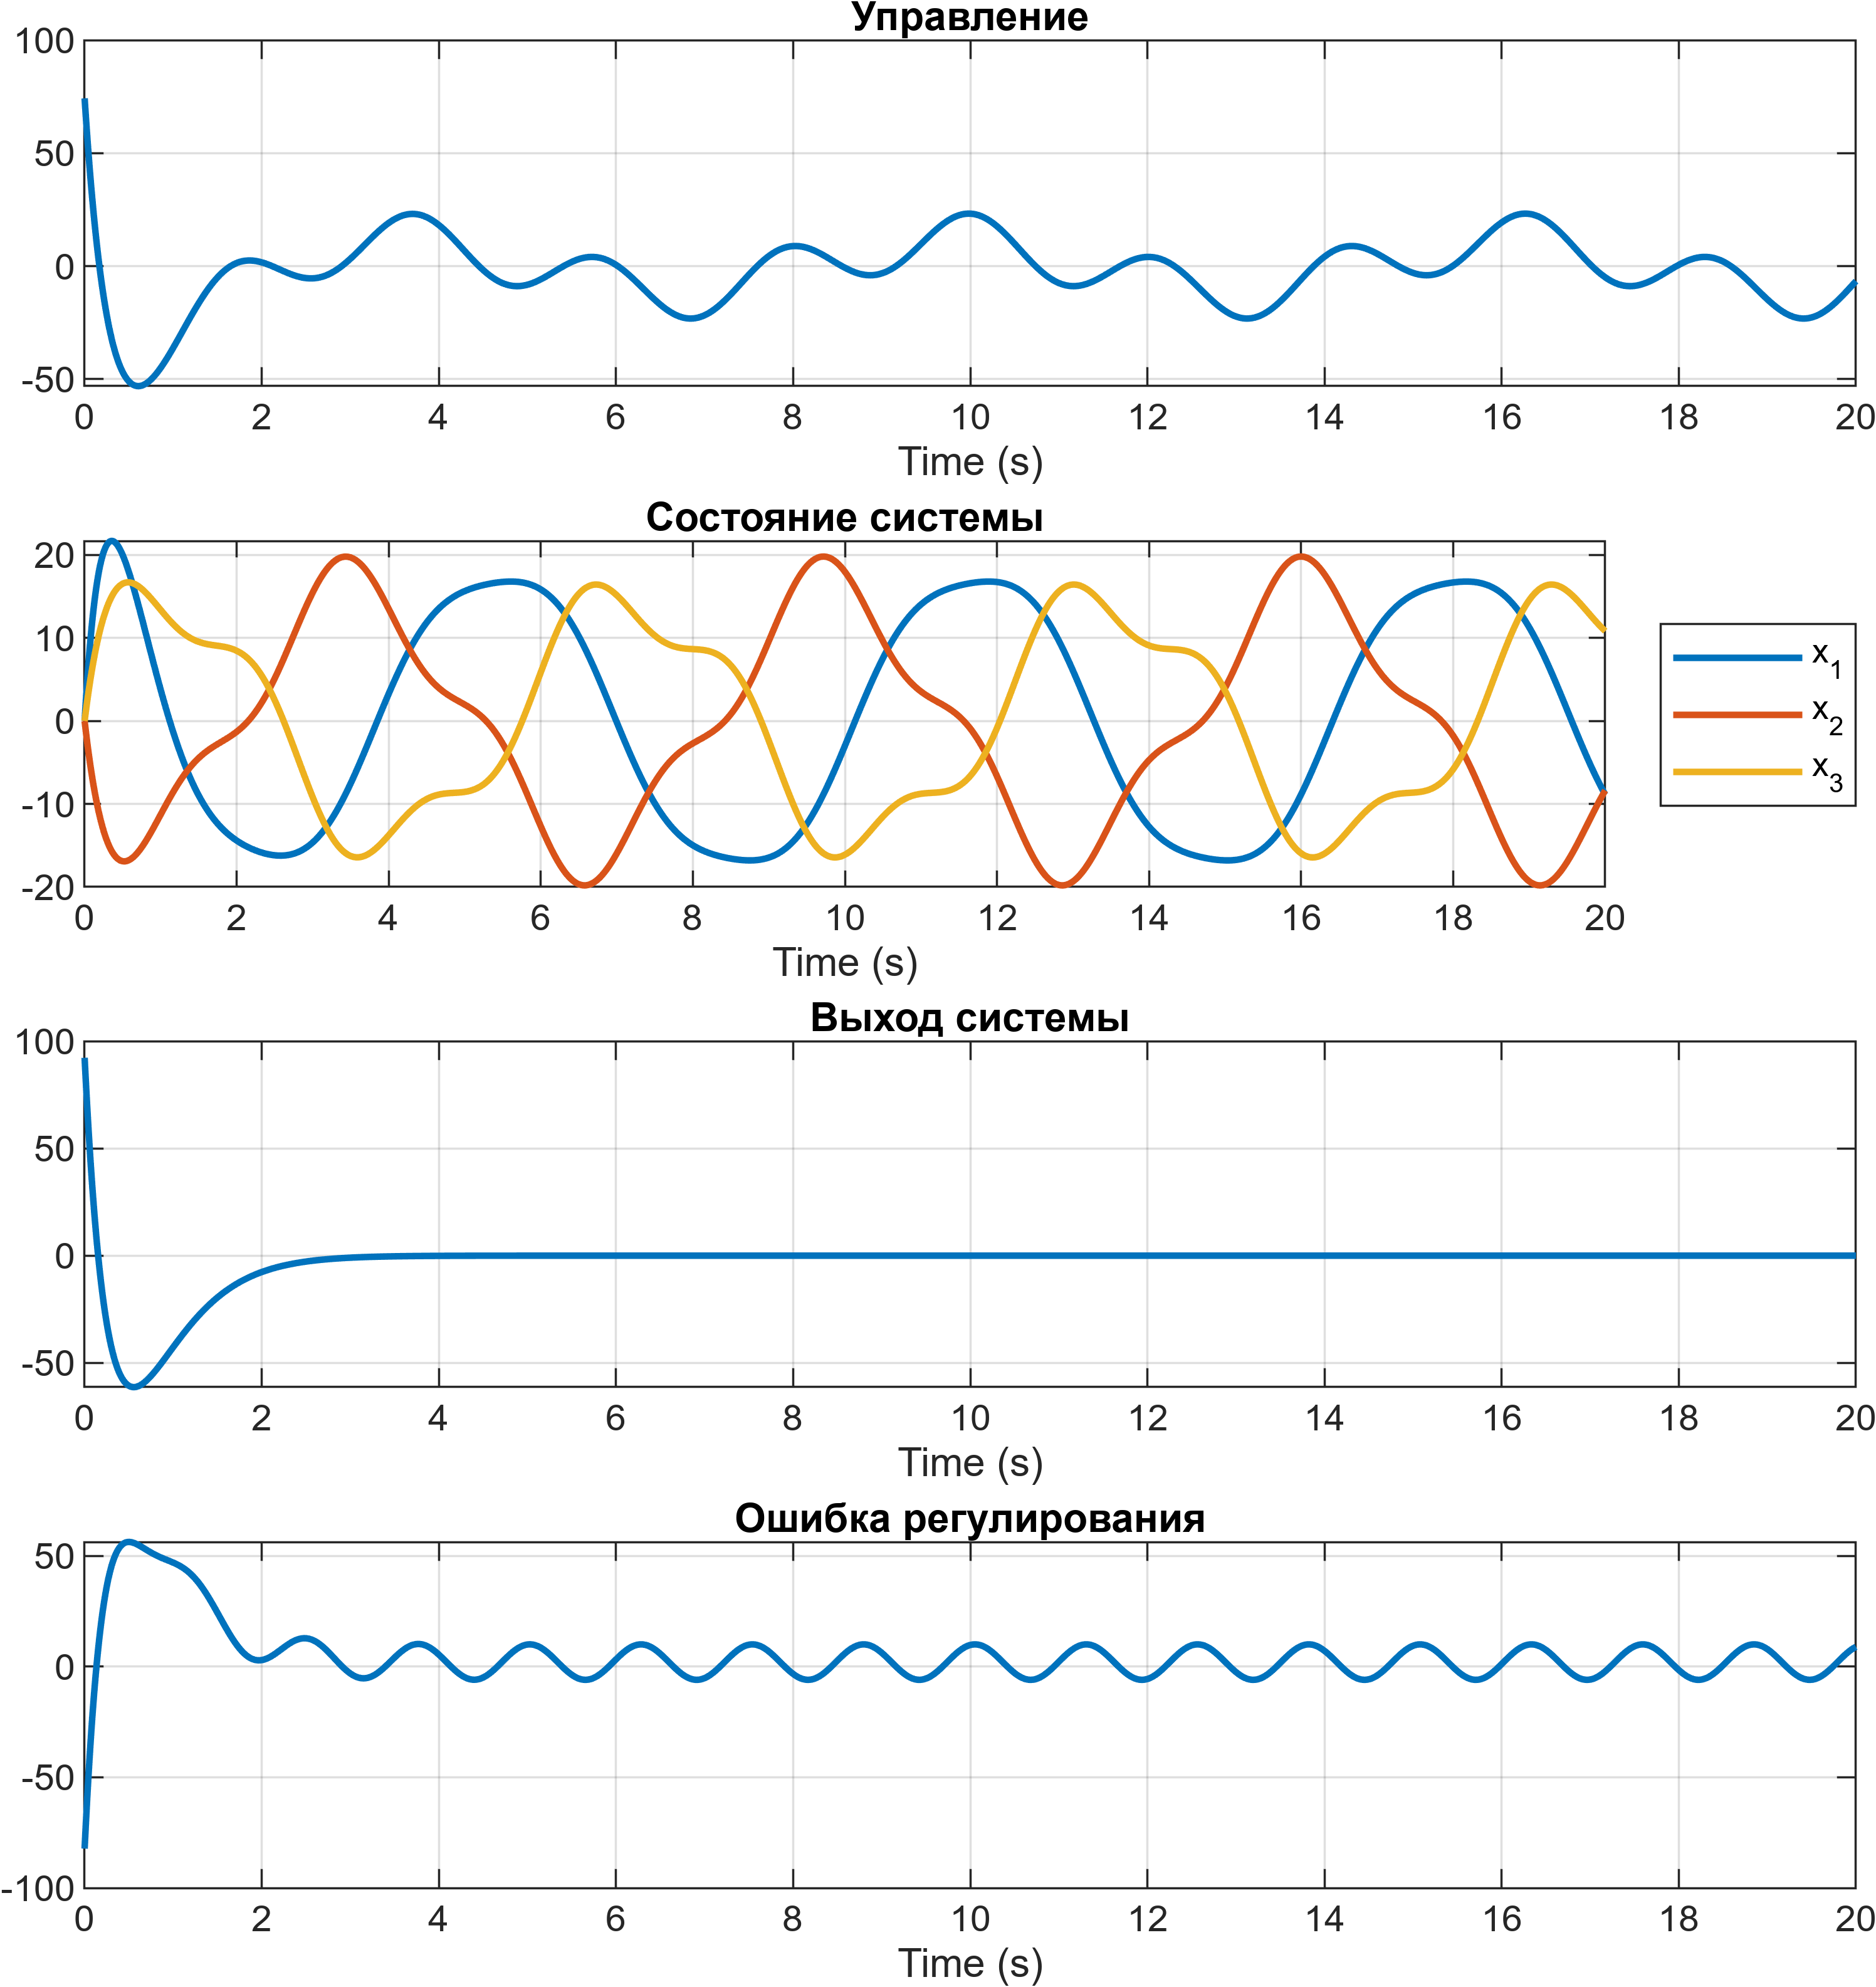
\includegraphics[width=\linewidth]{figs/12_sim.png}
    \caption{Замкнутая регулятором без следящей компоненты система \eqref{eq:sys1}}
    \label{fig:12sim}
\end{figure}
\begin{figure}[H]
    \centering
    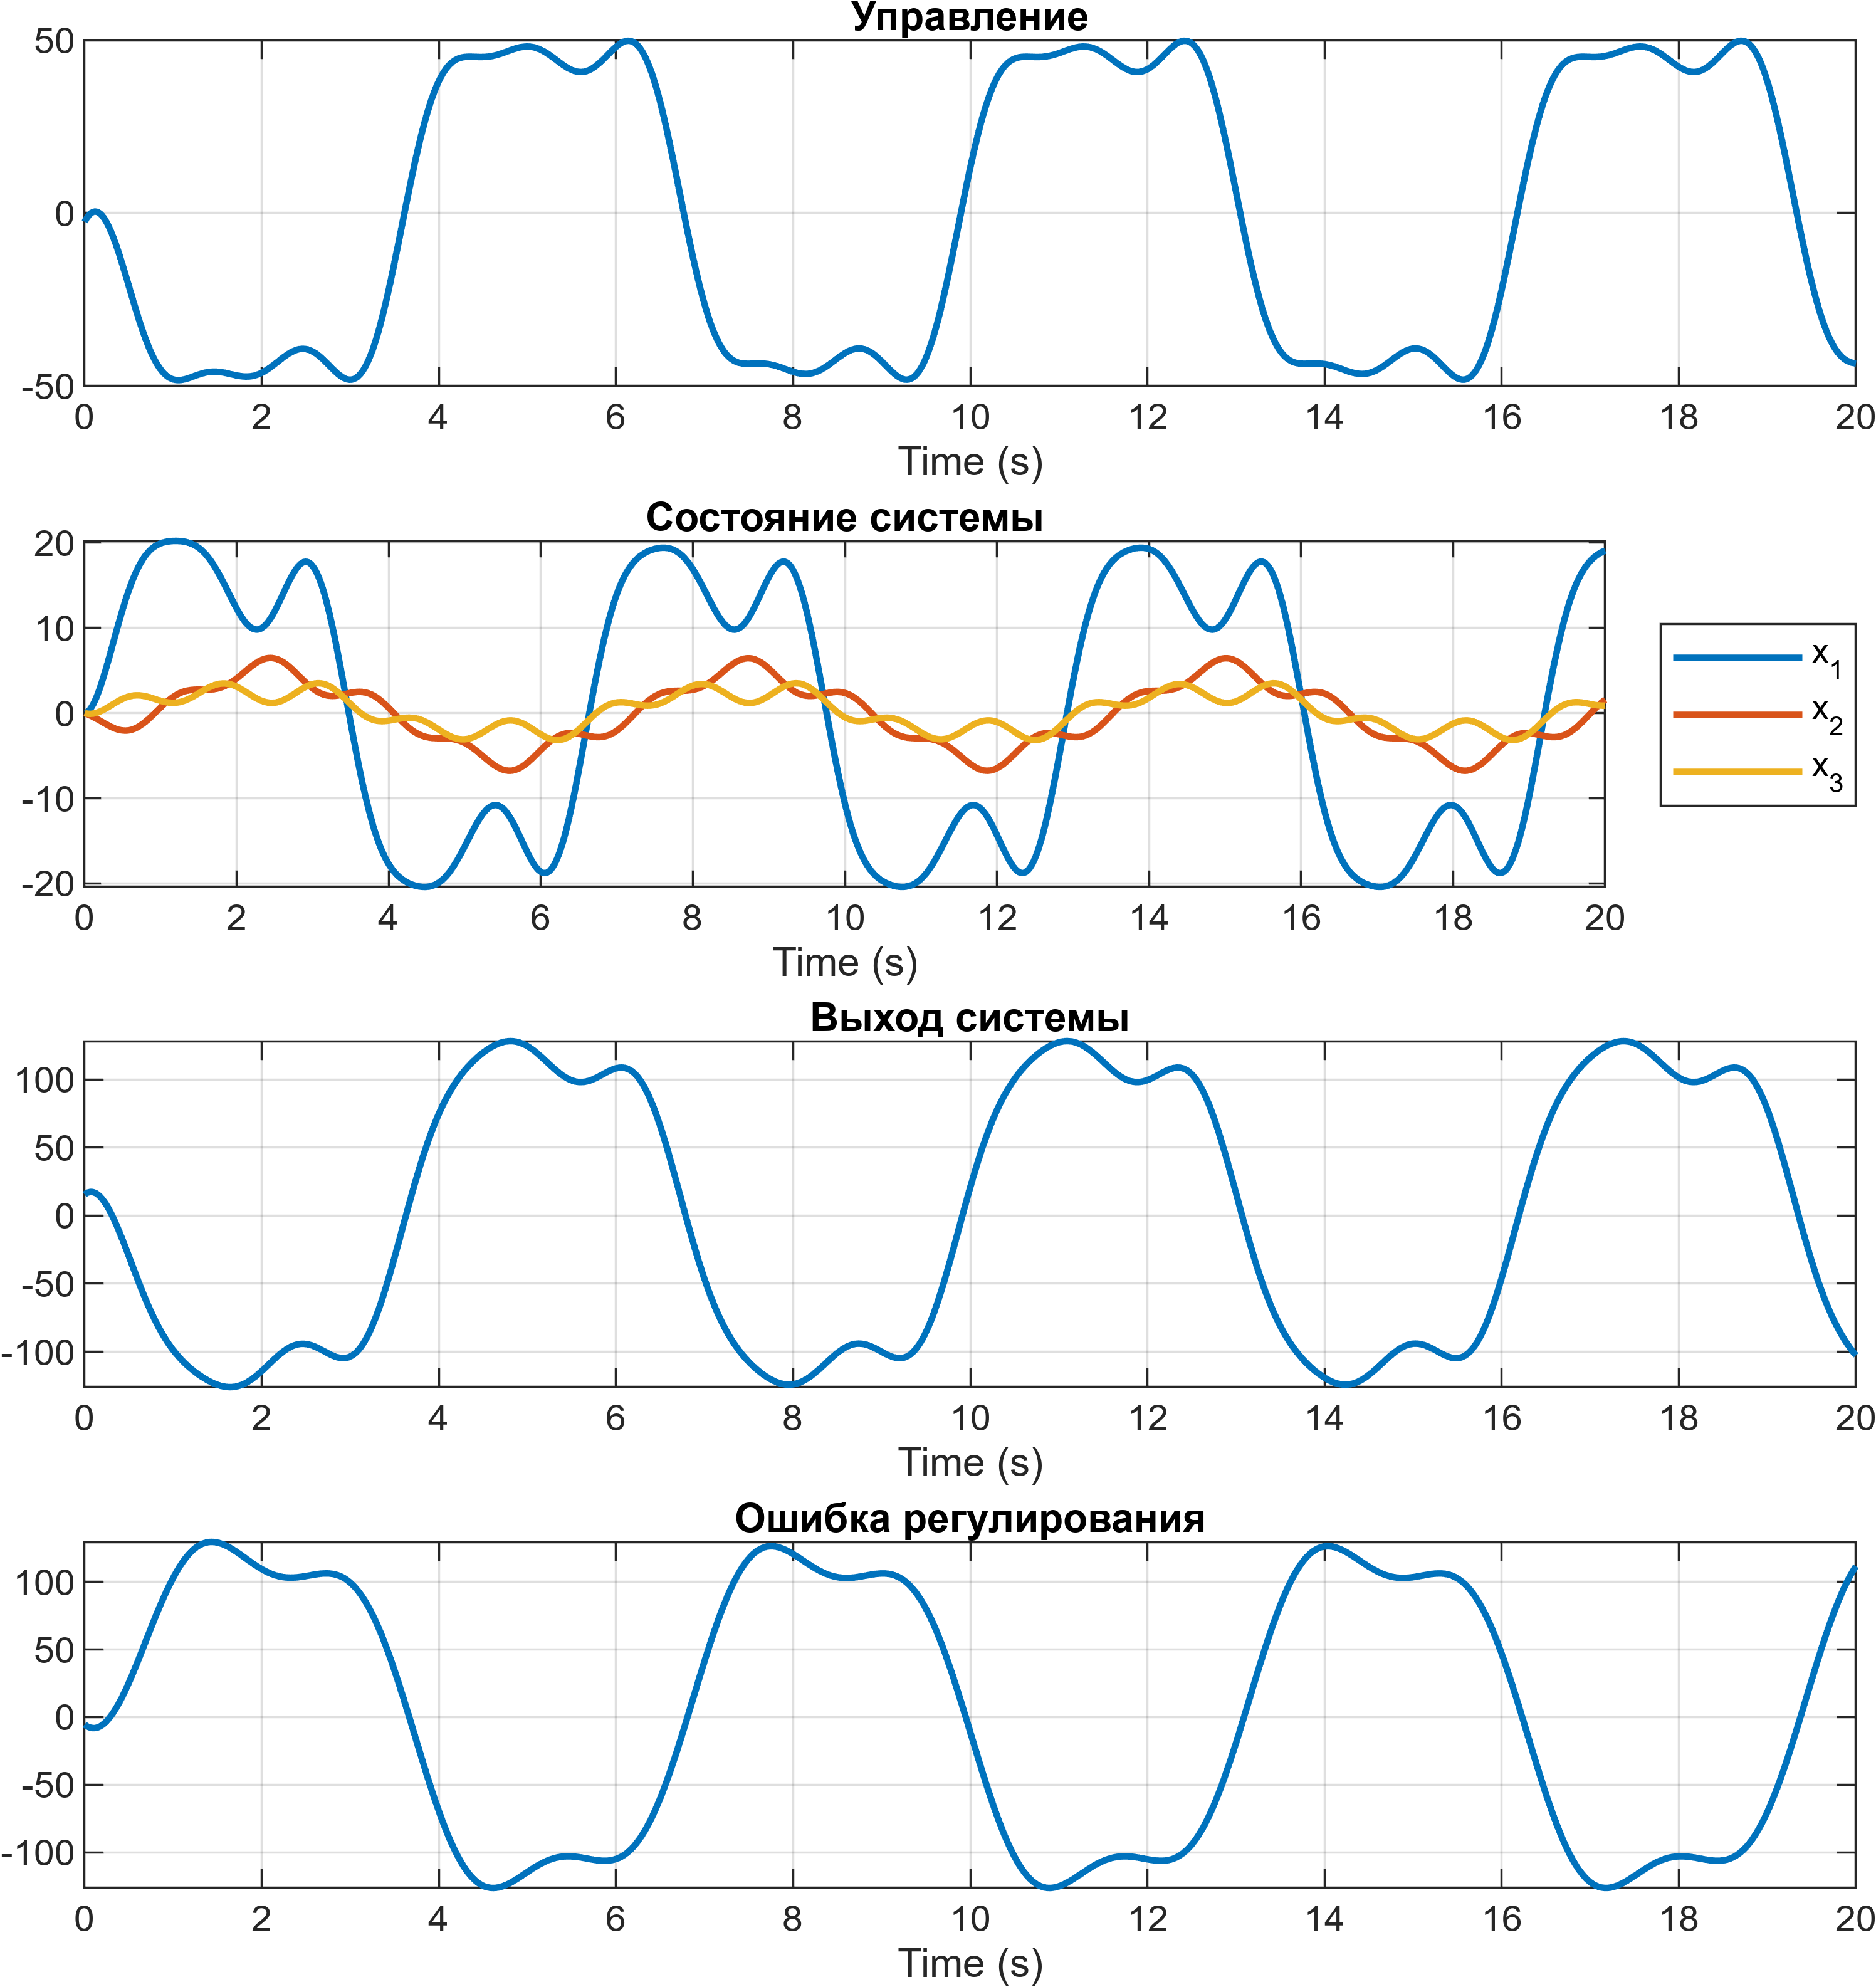
\includegraphics[width=\linewidth]{figs/13_sim.png}
    \caption{Замкнутая регулятором без компенсирующей компоненты система \eqref{eq:sys1}}
    \label{fig:13sim}
\end{figure}
\begin{figure}[H]
    \centering
    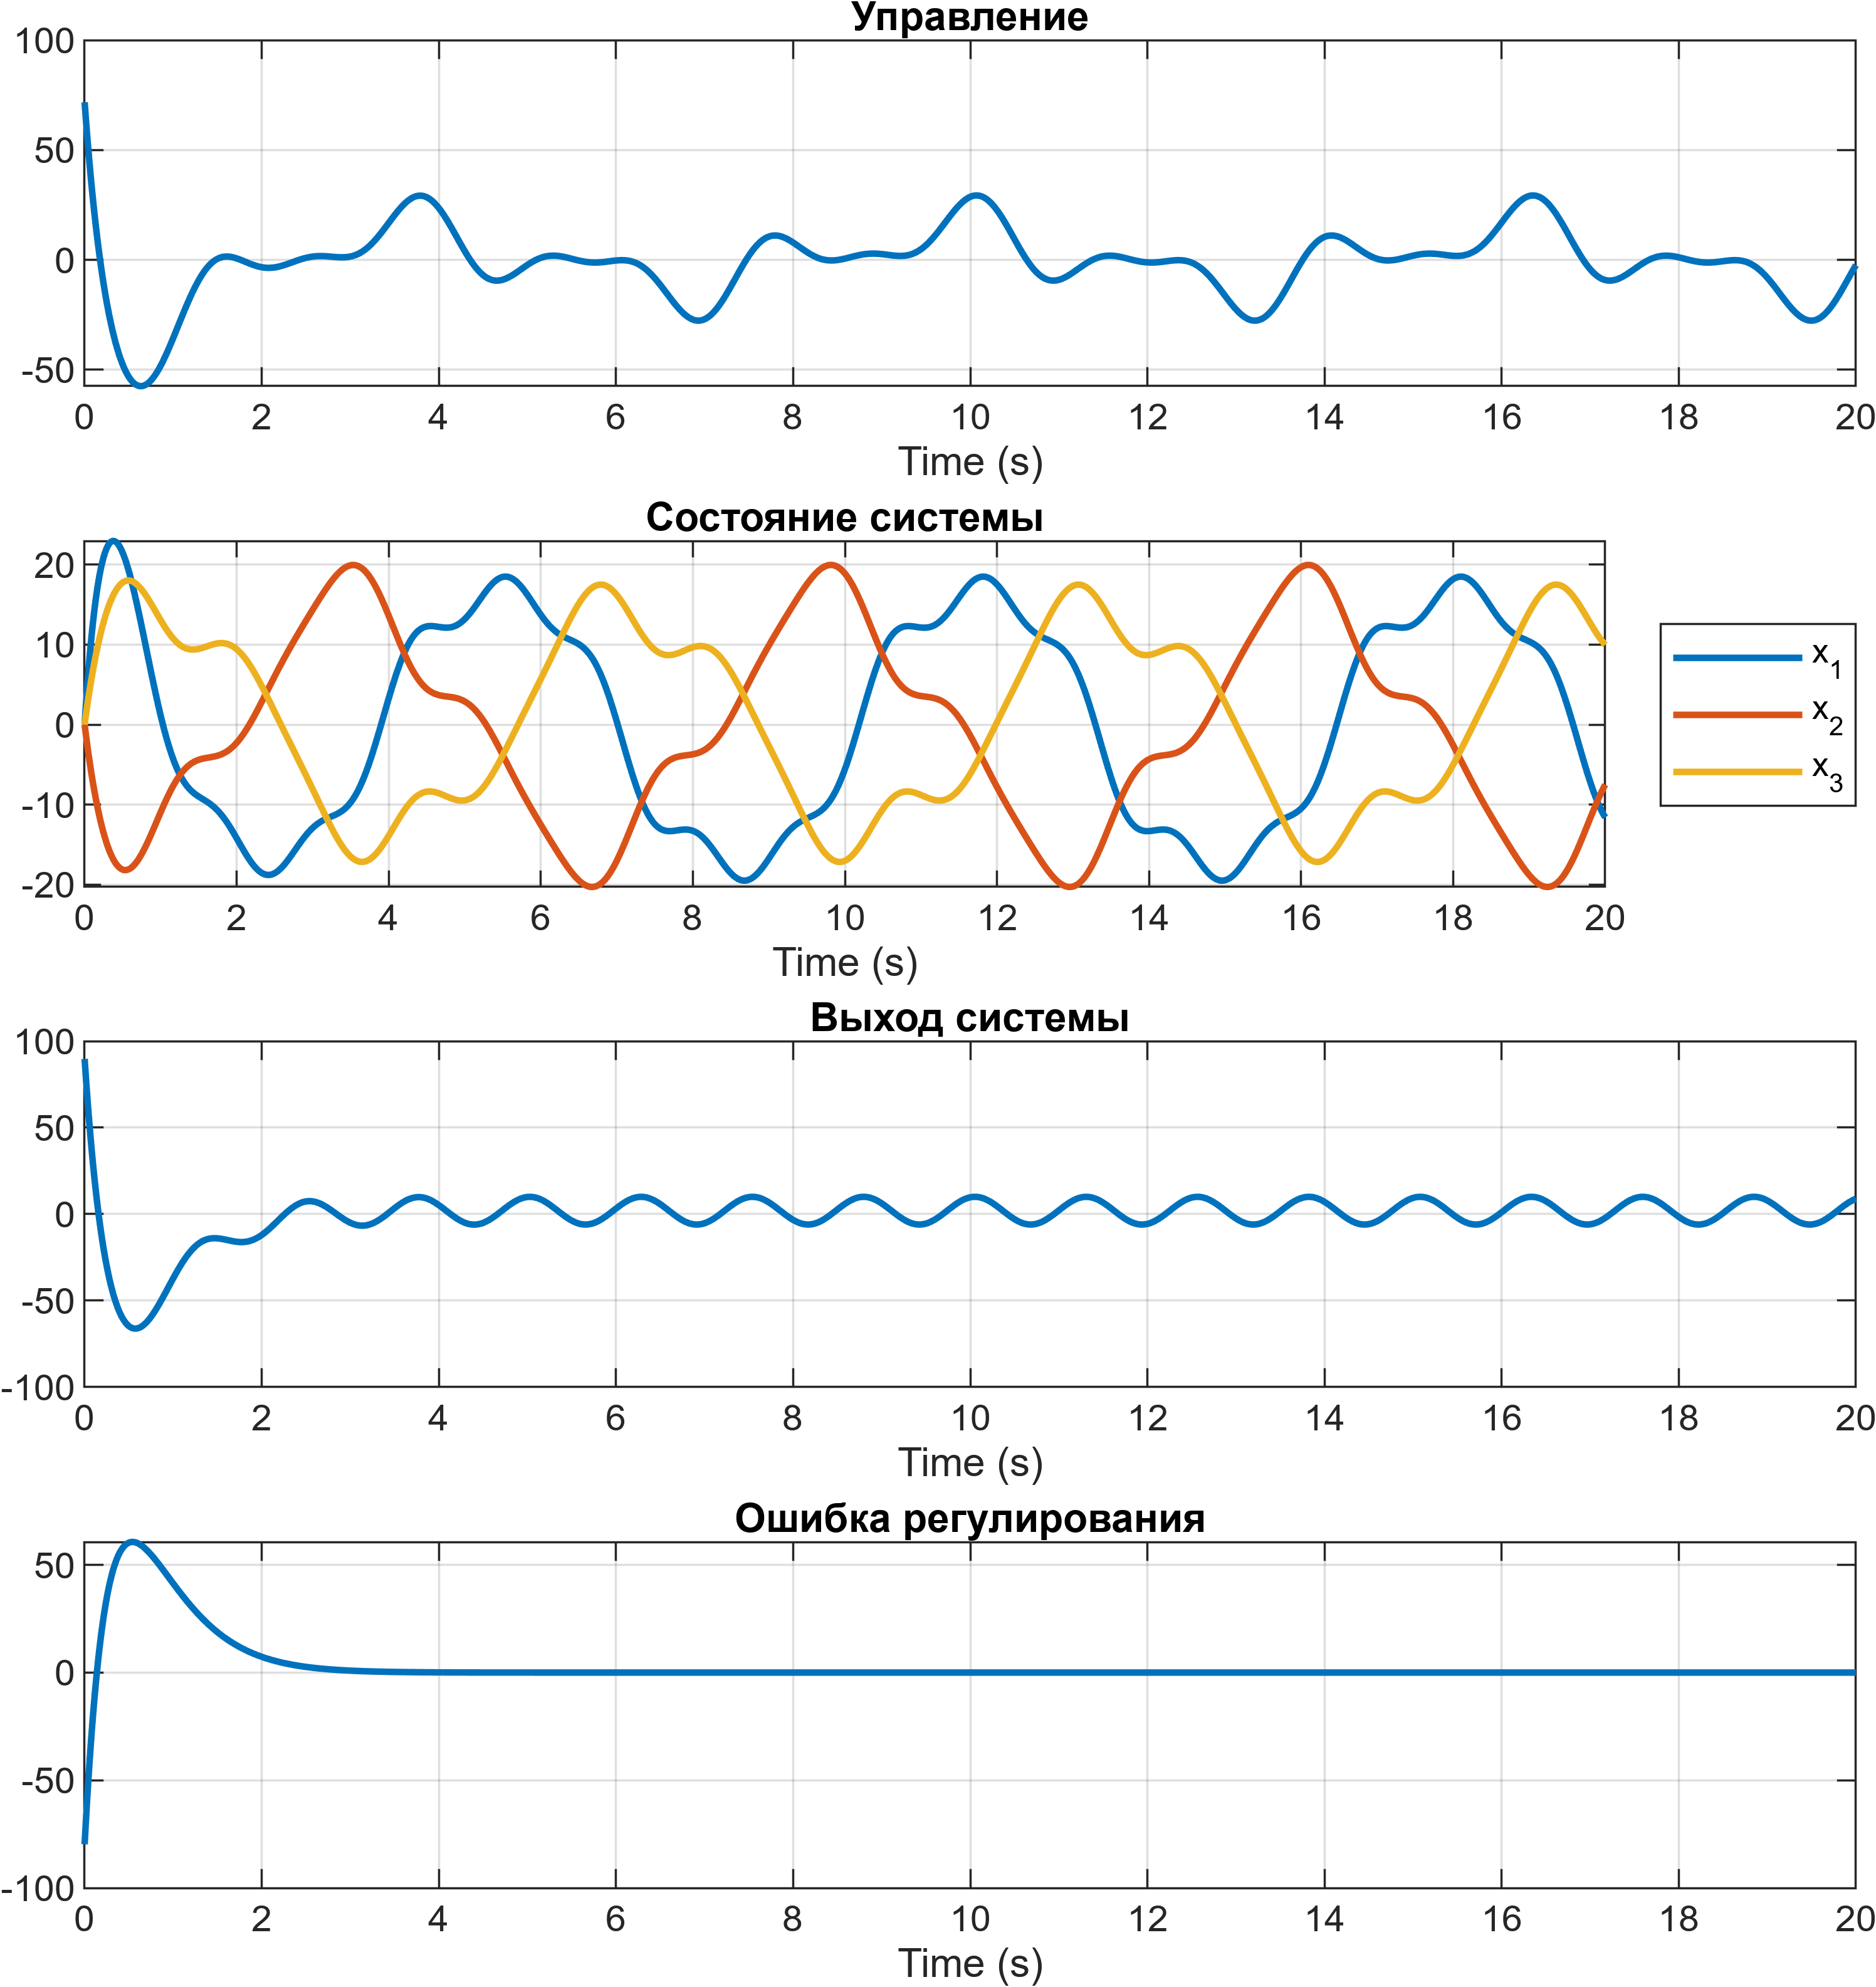
\includegraphics[width=\linewidth]{figs/14_sim.png}
    \caption{Замкнутая регулятором \eqref{eq:reg1} система \eqref{eq:sys1}}
    \label{fig:14sim}
\end{figure}

\subsection{Выводы}

В результате моделирования показано, что регулятор \eqref{eq:reg1} 
обеспечивает выполнение целевого условия \eqref{eq:goal1}. При разомкнутой системе
видно, что она неустойчива. При замкнутой только «feedback»-компонентой выход системы
колеблется под воздействием внешнего возмущения, и уже не уходит в бесконечность.
При замкнутой регулятором без следящей компоненты выход системы сошелся к нулю,
внешнее возмущение было успешно подавлено. При замкнутой регулятором без компенсирующей компоненты выход системы
колеблется под воздействием внешнего возмущения. При участии же весх трех слагаемых
регулятора \eqref{eq:reg1} выход системы идеально повторяет задающее воздействие.





\section{Слежение и компенсация по выходу}

\subsection{Структурная схема}

\begin{figure}[H]
    \centering
    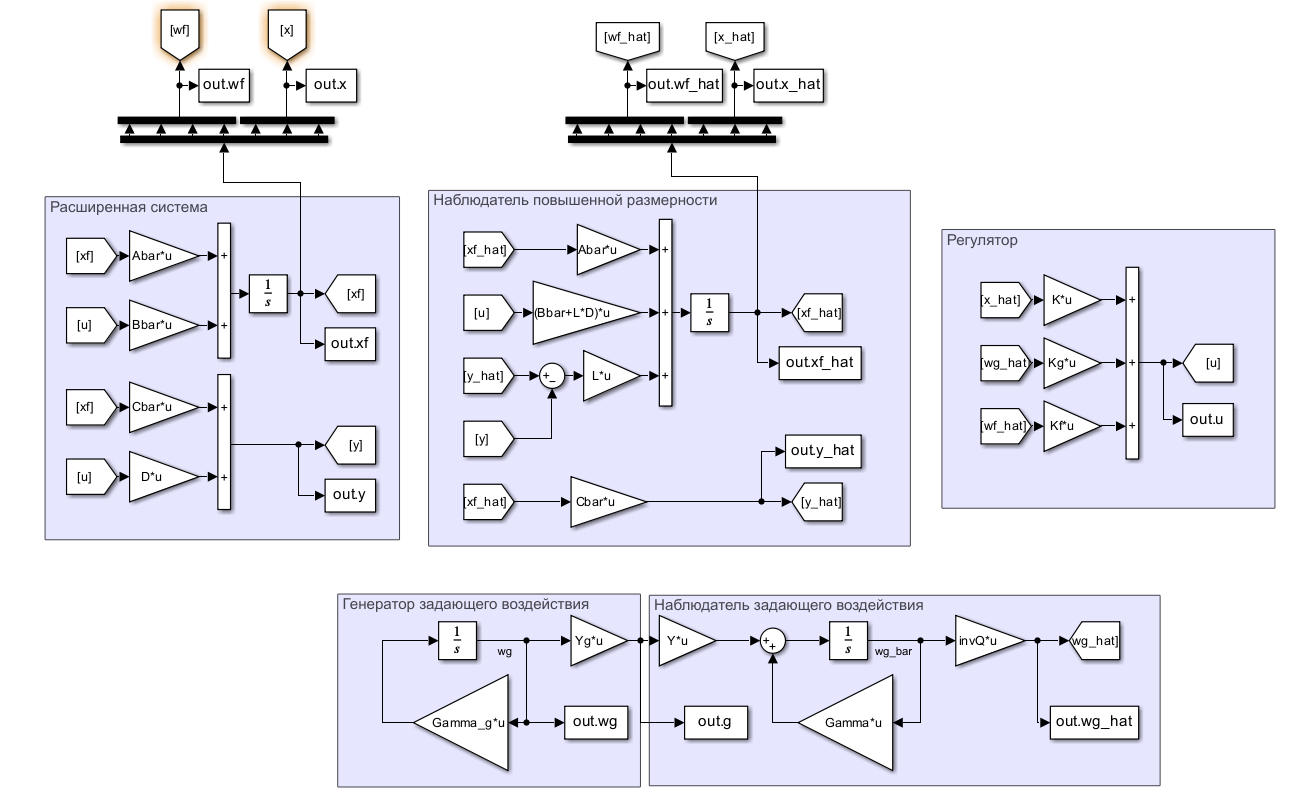
\includegraphics[width=\linewidth]{figs/20slx.png}
    \caption{Схема моделирования системы \eqref{eq:sys1}, замкнутой регулятором, состоящим
    из наблюдателя задающего воздействия, наблюдателя расширенной размерности
    и закона управления \eqref{eq:reg2}}
    \label{fig:sys2}
\end{figure}

Построим моделирования системы \eqref{eq:sys1}, замкнутой регулятором, состоящим
из наблюдателя задающего воздействия, наблюдателя расширенной размерности
и закона управления
\begin{equation}
    \label{eq:reg2}
    u=K\hat x+K_g\hat w_g+K_f\hat w_f,
\end{equation}
обеспечивающим выполнение целевого условия \eqref{eq:goal1}.

\subsection{Синтез наблюдателя}

Синтезируем наблюдатель задающего воздействия, для этого необходимо решить
уравнение Ляпунова:
\begin{equation}
    \label{eq:lyap1}
    Q\Gamma_g-\Gamma Q=YY_g
\end{equation}
относительно $Q$, где $\Gamma_g$ и $Y_g$ из \eqref{eq:sys1g}, а
$\Gamma$ и $Y$ подберем таким образом, чтобы $\Gamma$ была Грувицева,
спектры $\Gamma$ и $\Gamma_g$ не пересекались, $(\Gamma,\ Y)$ - управляема, $(\Gamma_g,\ Y_g)$ уже наблюдаема. 
Тогда
\begin{equation*}
    \Gamma=\begin{bmatrix}
        -2 & 0 & 0 \\
        0 & -3 & 0 \\
        0 & 0 & -4
    \end{bmatrix},\quad
    Y=\begin{bmatrix}
        1 \\ 1 \\ 1
    \end{bmatrix}.
\end{equation*}
С помощью CVX в MATLAB получили:
\begin{equation*}
    Q=\begin{bmatrix}
        0.5517&	-1.3793&	1.0000\\
        0.7059&	-1.1765&	0.6667\\
        0.7805&	-0.9756&	0.5000
    \end{bmatrix}.
\end{equation*}
Эта матрица $Q$ является матрицой перехода наблюдателя:
\begin{equation*}
    \bar w_g=Q\hat w_g.
\end{equation*}

\subsection{Синтез наблюдателя расширенной размерности}

Введем расширенную систему:
\begin{equation}
    \label{eq:sys2}
    \begin{cases}
        \dot x_f=\bar Ax_f+\bar B u\\
        y=\bar Cx_f+Du
    \end{cases},
\end{equation}
где
\begin{equation*}
    x_f=\begin{bmatrix}
        w_f\\x
    \end{bmatrix},\quad
    \bar A=\begin{bmatrix}
        \Gamma_f & 0 \\
        B_fY_f & A
    \end{bmatrix},\quad
    \bar B=\begin{bmatrix}
        0\\0\\0\\0\\B
    \end{bmatrix},\quad
    \bar C=\begin{bmatrix}
        D_fY_f&C
    \end{bmatrix},
\end{equation*}
и наблюдатель повышенной размерности:
\begin{equation*}
    \label{eq:obs2}
    \begin{cases}
        \dot{\hat x}_f=\bar A\hat x_f+(\bar B+LD) u+L(\hat y-y)\\
        \hat y=\bar C\hat x_f
    \end{cases}.
\end{equation*}
Найдем матрицу $L$ через решение уравнения Сильвестра 
\begin{equation*}
    Q\bar A-\Gamma Q=Y \bar C,\quad L=-Q^{-1}Y.
\end{equation*}
Спектр $\bar A$:
\begin{equation*}
    \sigma(\bar A)=\{
        -0.0000 \pm 3.0000i,\ 
-2.0000 + 0.0000i,\ 
2.0000 \pm 1.0000i,\ 
0.0000 \pm 1.0000i
    \}.
\end{equation*}
Выберем следущием матрицы:
\begin{equation*}
    \Gamma=\begin{bmatrix}
        -1 & 0 & 0 & 0 & 0 & 0 & 0 \\
        0 & -3 & 0 & 0 & 0 & 0 & 0 \\
        0 & 0 & -4 & 0 & 0 & 0 & 0 \\
        0 & 0 & 0 & -5 & 0 & 0 & 0 \\
        0 & 0 & 0 & 0 & -6 & 0 & 0 \\
        0 & 0 & 0 & 0 & 0 & -7 & 0 \\
        0 & 0 & 0 & 0 & 0 & 0 & -8
    \end{bmatrix},\quad
    Y=\begin{bmatrix}
        1 \\ 1 \\ 1 \\ 1 \\ 1 \\ 1 \\ 1
    \end{bmatrix}.
\end{equation*}
Выполнены следующие условия существования решения: спектры $\bar A$ и $\Gamma$ не пересекаются,
$(\bar A,\ \bar C)$ - наблюдаема, $(Y,\ \Gamma)$ - управляема. С помощью CVX
получили:
\begin{equation*}
    L=\begin{bmatrix}
        -298.14&
        184.32&
        -51.62&
        -30.63&
        -885.09&
        1835.49&
        -1839.02
    \end{bmatrix}^T.
\end{equation*}

\subsection{Компьютерное моделирование}

Проведено моделирование системы \eqref{eq:sys1}, 
замкнутой регулятором \eqref{eq:reg2}, с наблюдателем задающего
воздействия, наблюдателем расширенной размерности. 
Построены следующие графики:
\begin{itemize}
    \item Графики управления $u(t)$, выхода $y(t)$ и ошибки слежения 
    $e(t)=y(t)-g(t)$ представлены на \autoref{fig:20}.
    \item Графики внешнего возмущения $w_f(t)$, состояния $x(t)$ и 
    их оценок из расширенного наблюдателя показаны на \autoref{fig:21}.
    \item Графики ошибки между внешним воздействием и его оценкой $w_f-\hat w_f$, 
    состояния системы и его оценкой $x-\hat x$ приведены на \autoref{fig:22}.
    \item Графики задающего воздействия $w_g(t)$, его оценки $\hat w_g(t)$ и 
    ошибки наблюдения $w_g(t)-\hat w_g(t)$ представлены на \autoref{fig:23}.
\end{itemize}

\begin{figure}[H]
    \centering
    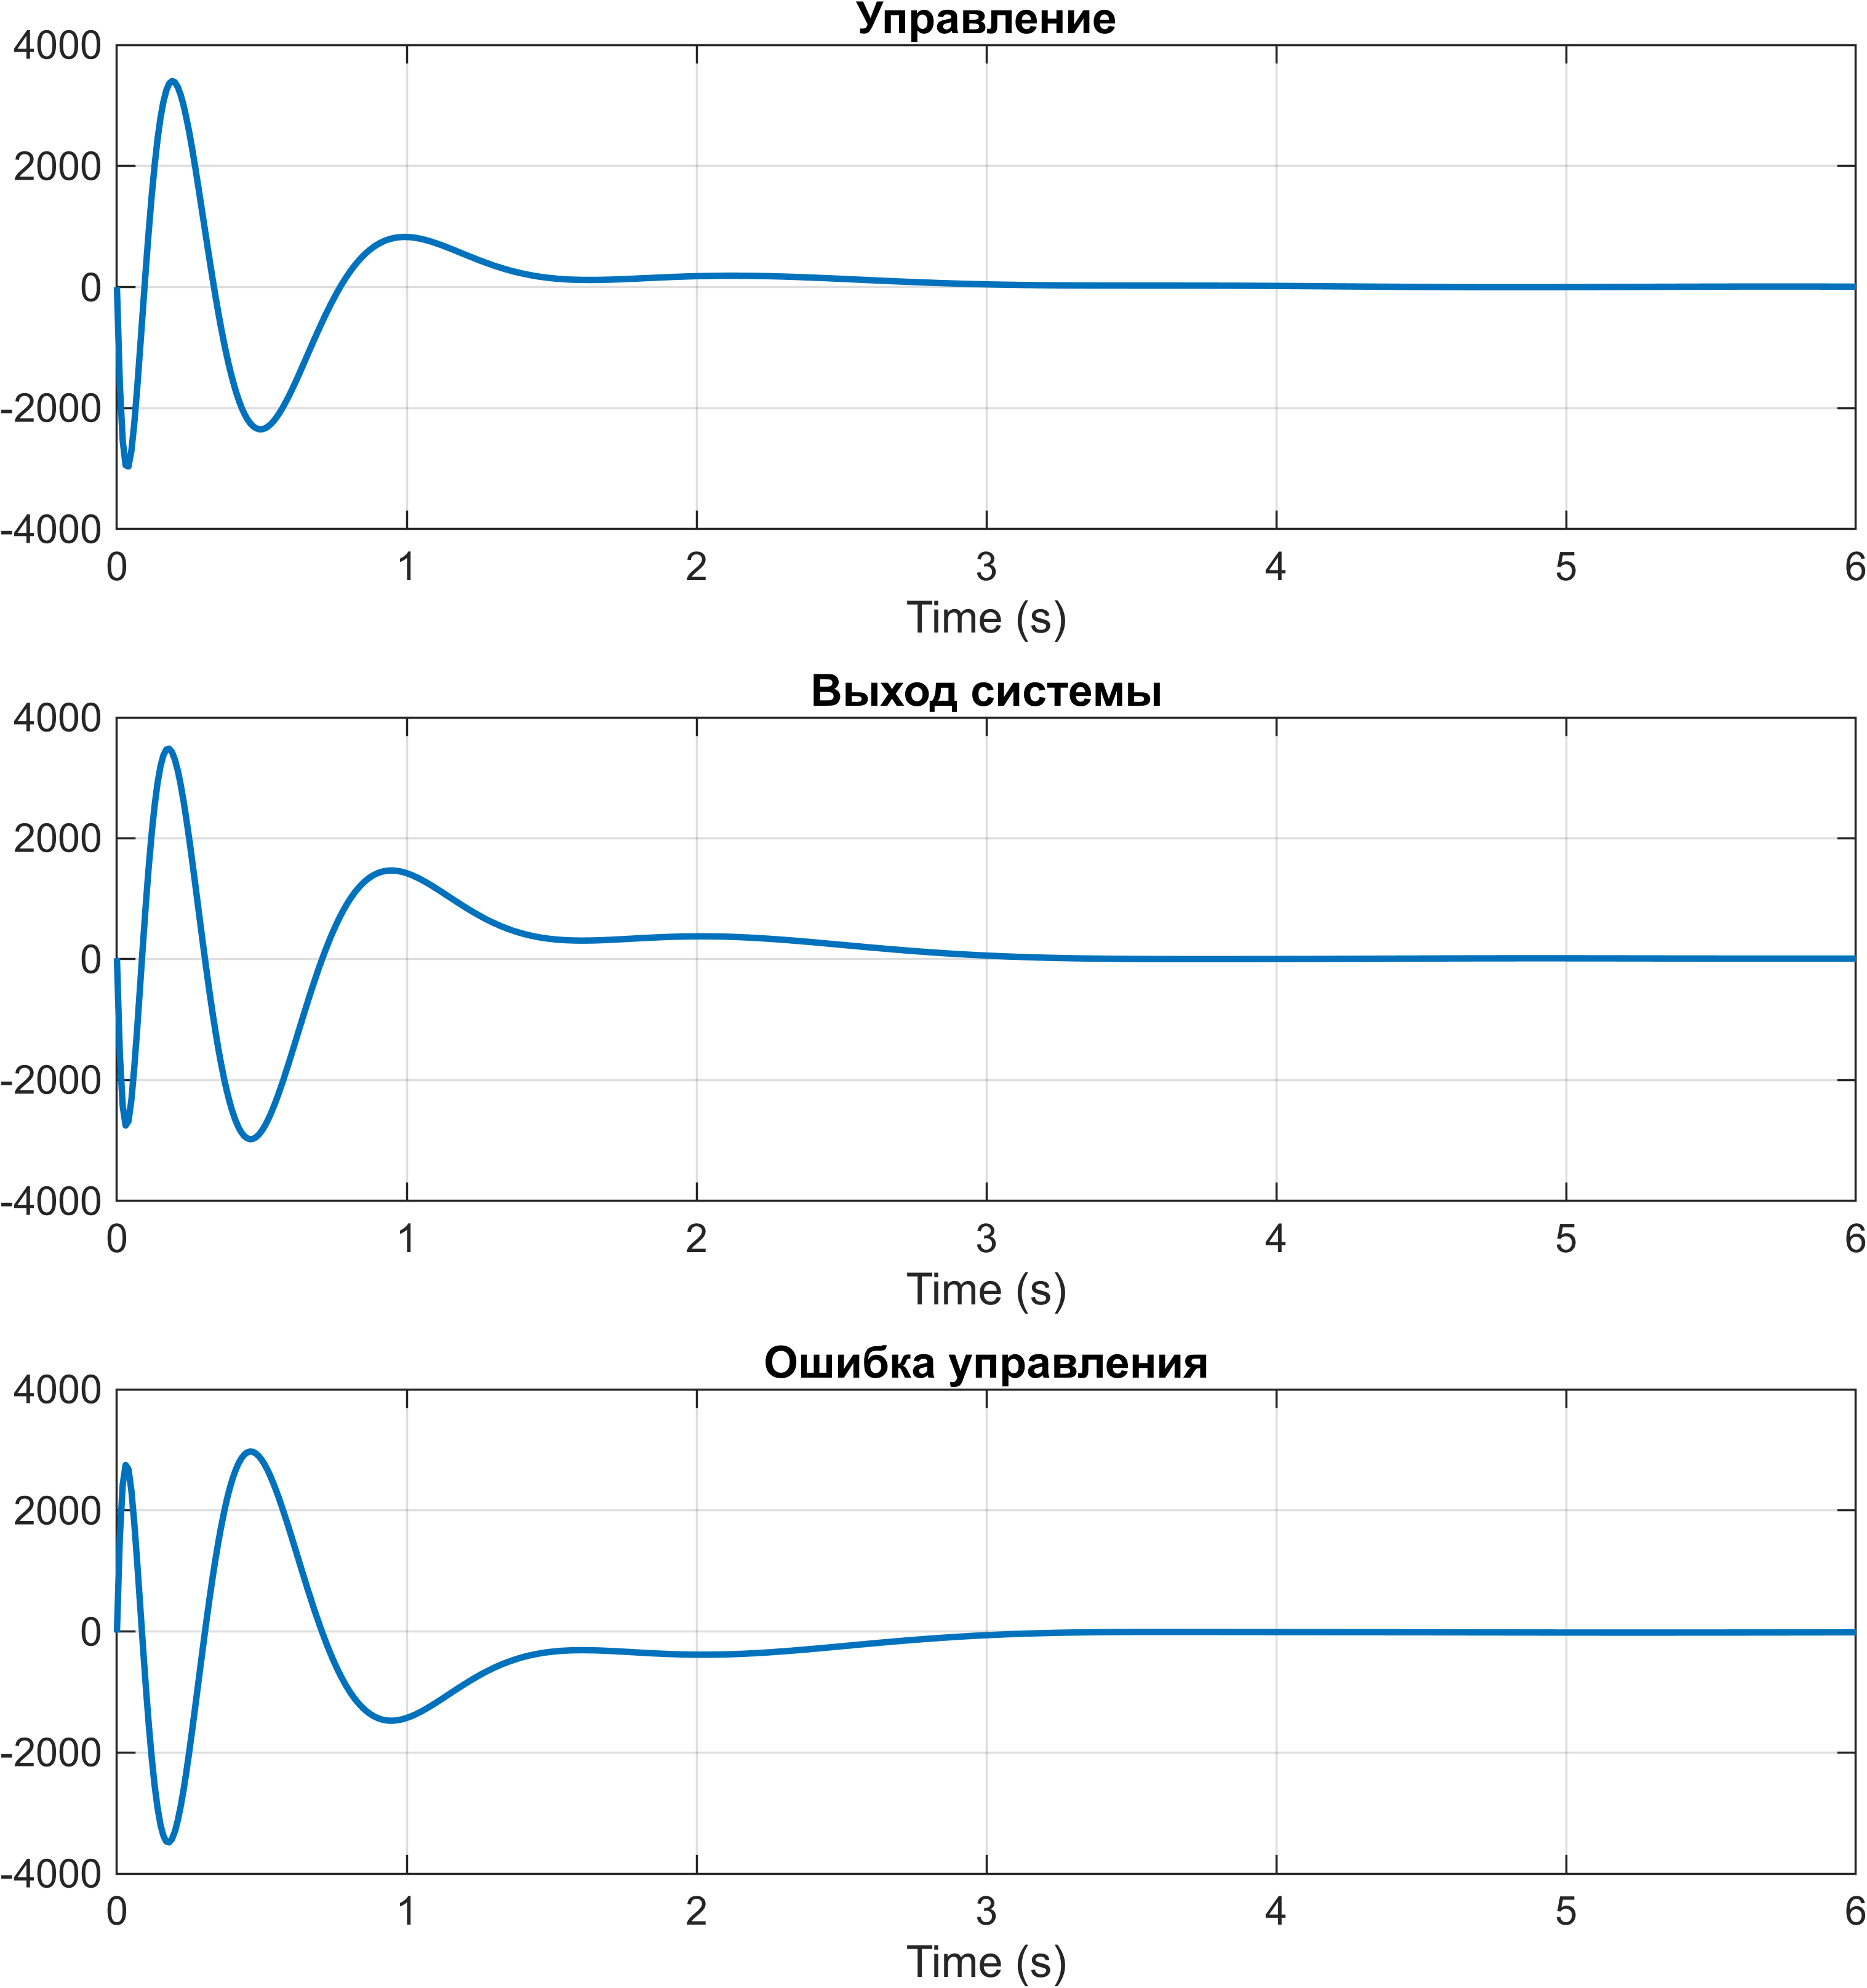
\includegraphics[width=\linewidth]{figs/20_sim.png}
    \caption{Графики управления $u(t)$, выхода $y(t)$ и ошибки слежения
    $e(t)=y(t)-g(t)$}
    \label{fig:20}
\end{figure}

\begin{figure}[H]
    \centering
    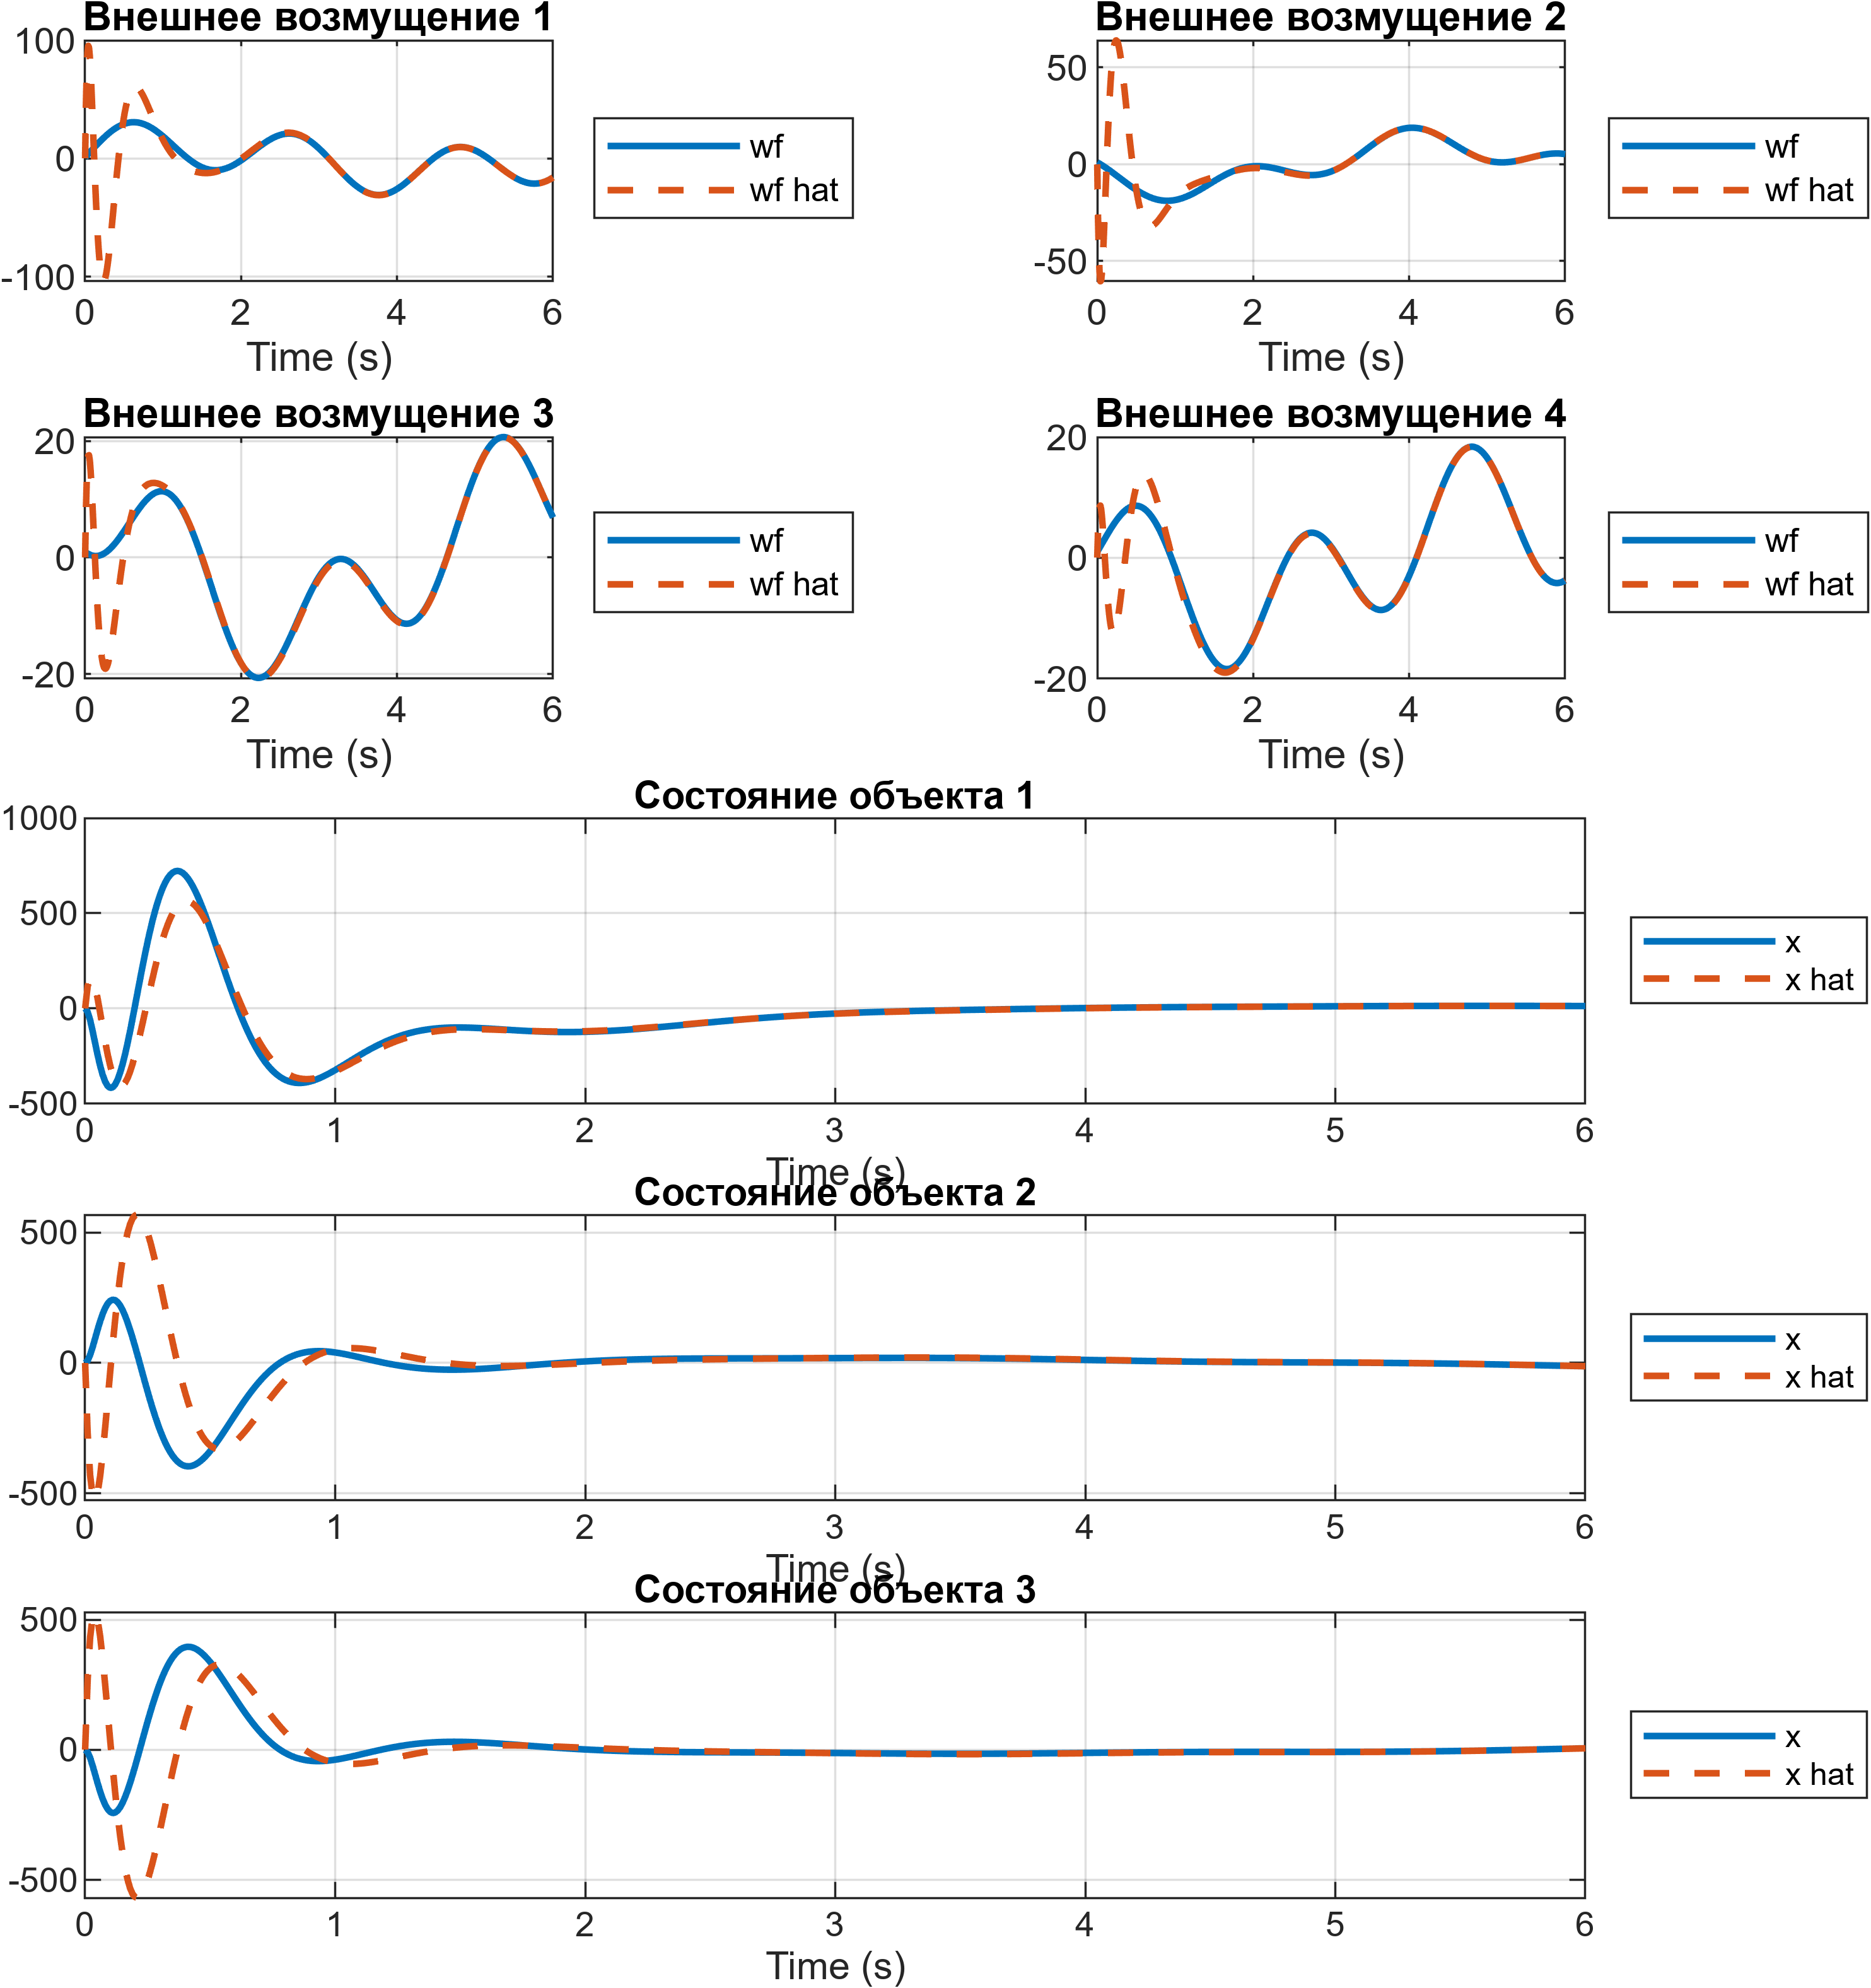
\includegraphics[width=\linewidth]{figs/21_sim.png}
    \caption{Графики внешнего возмущения $w_f(t)$, состояния $x(t)$ и их оценок
    из расширенного наблюдателя}
    \label{fig:21}
\end{figure}

\begin{figure}[H]
    \centering
    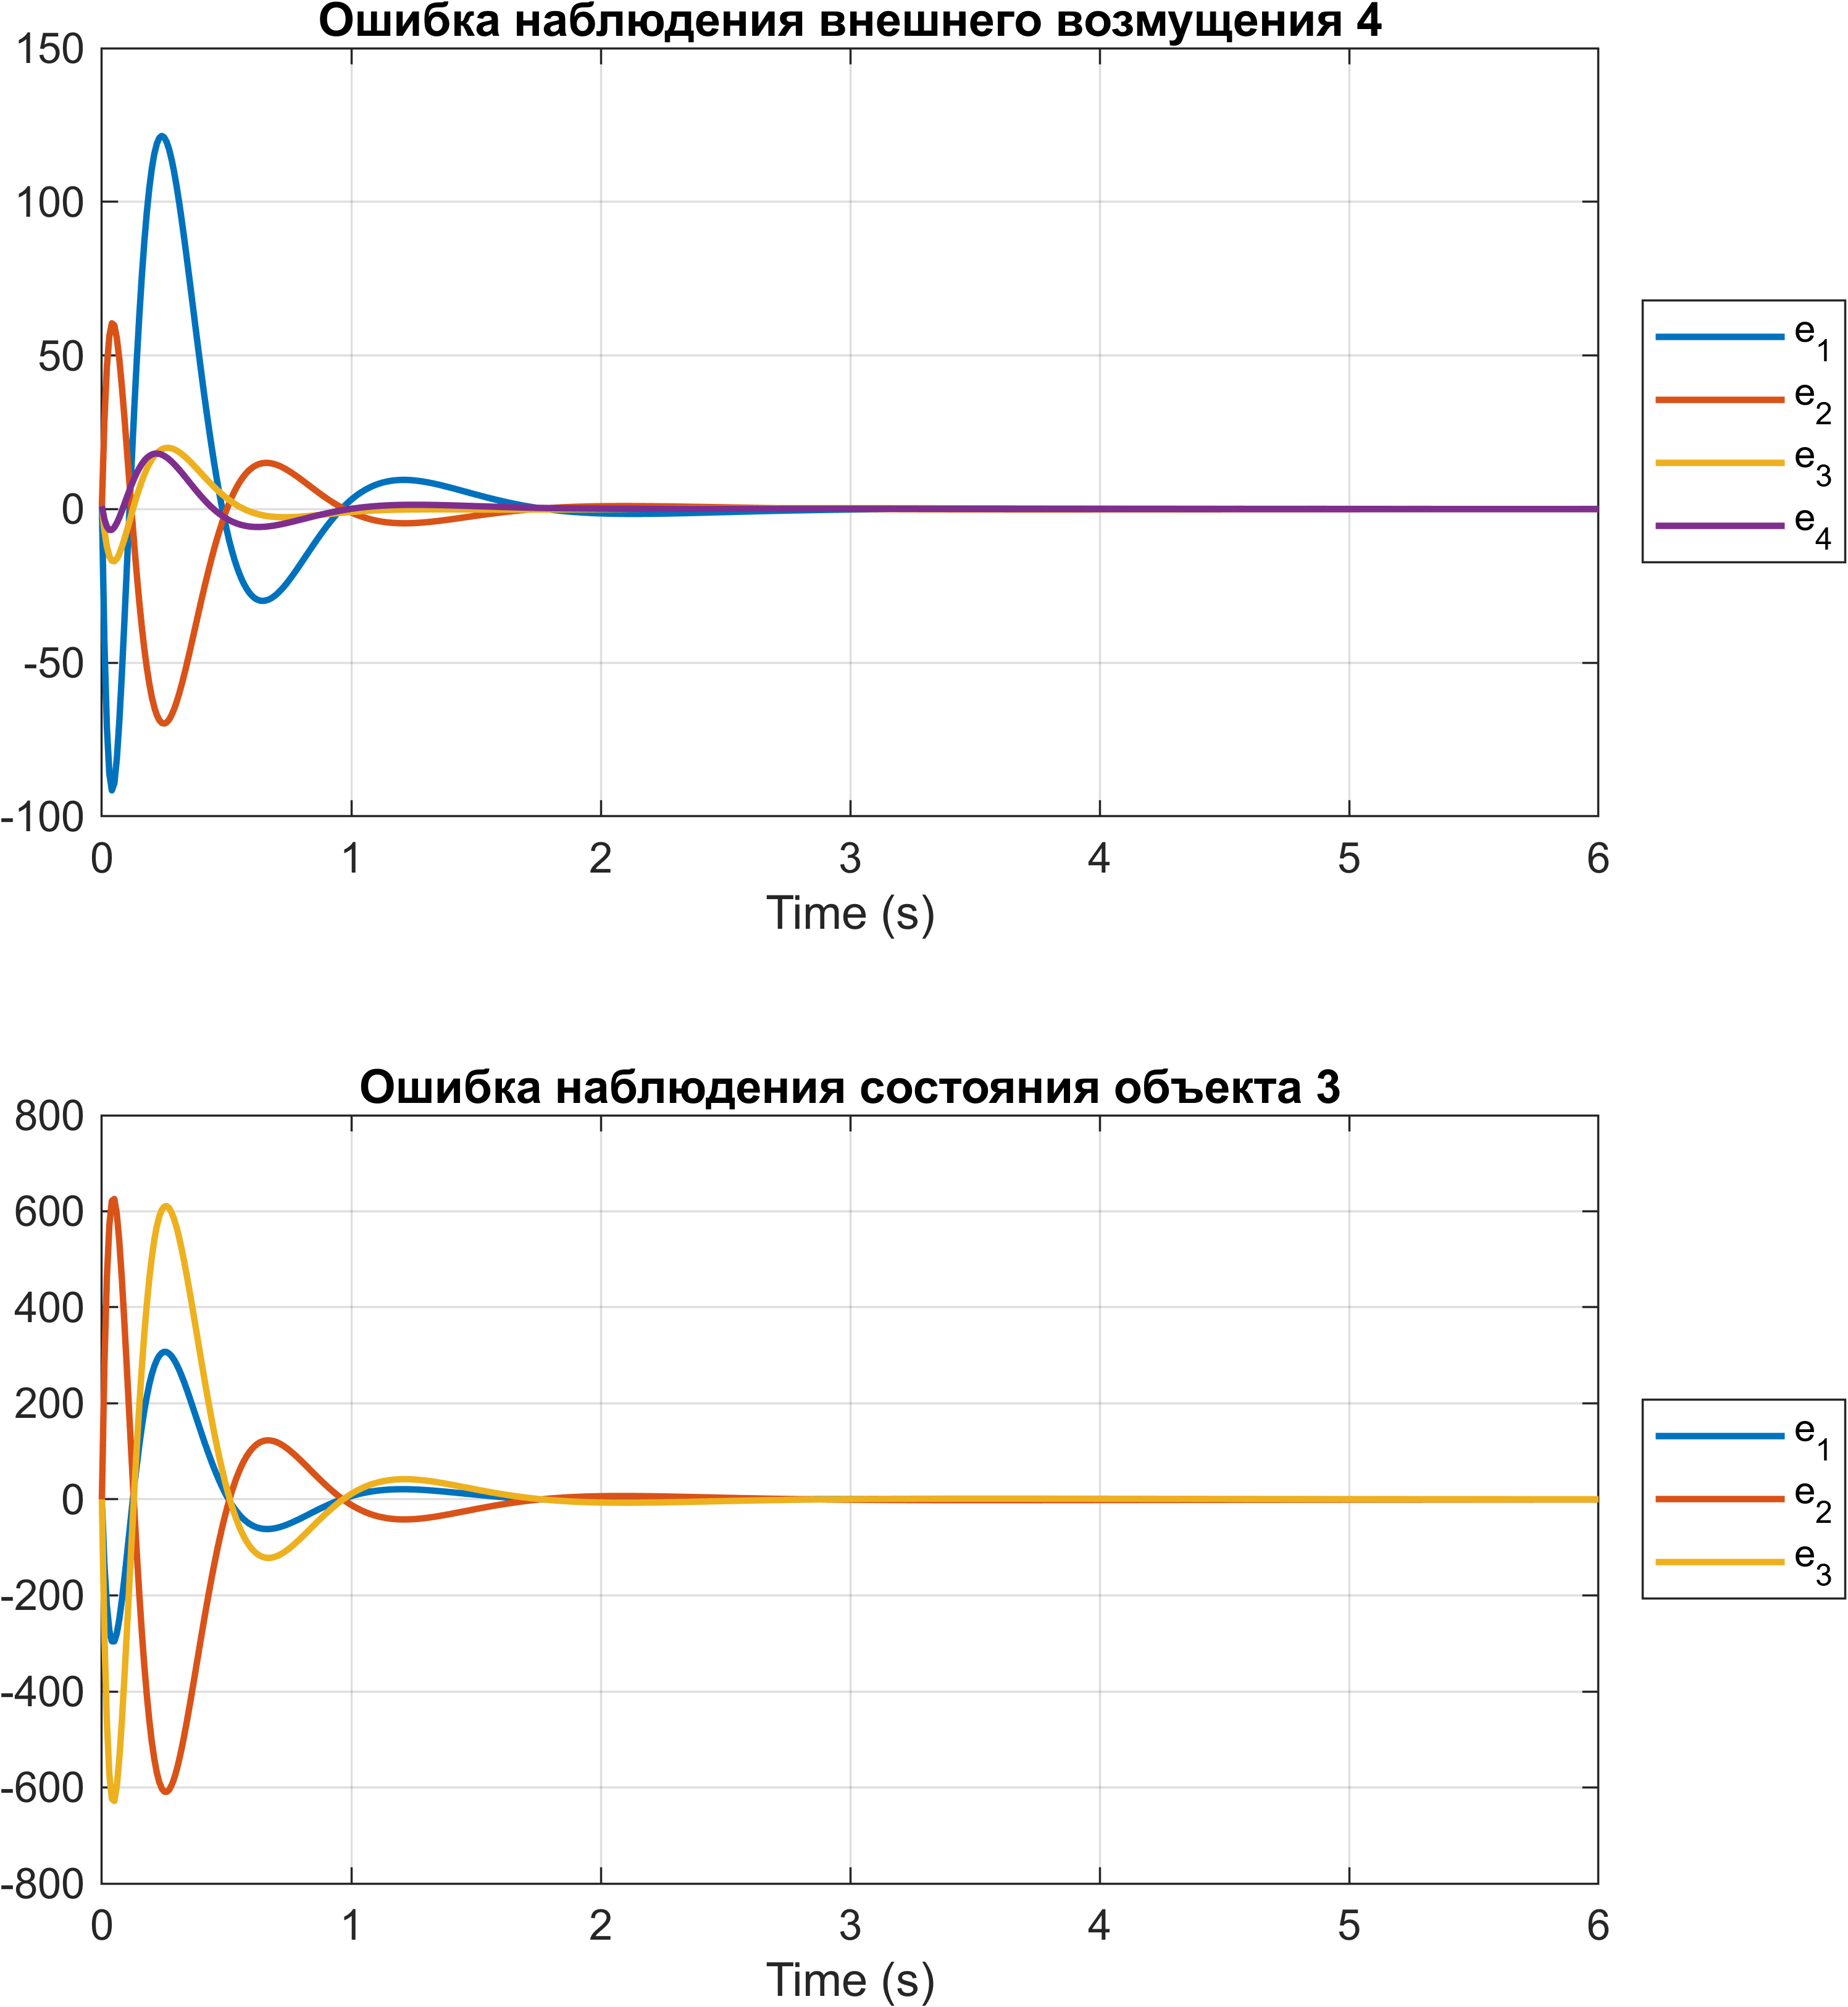
\includegraphics[width=\linewidth]{figs/22_sim.png}
    \caption{Графики ошибки между внешним воздействие и его оценкой $w_f-\hat w_f$,
    состояния системы и его оценкой $x-\hat x$}
    \label{fig:22}
\end{figure}

\begin{figure}[H]
    \centering
    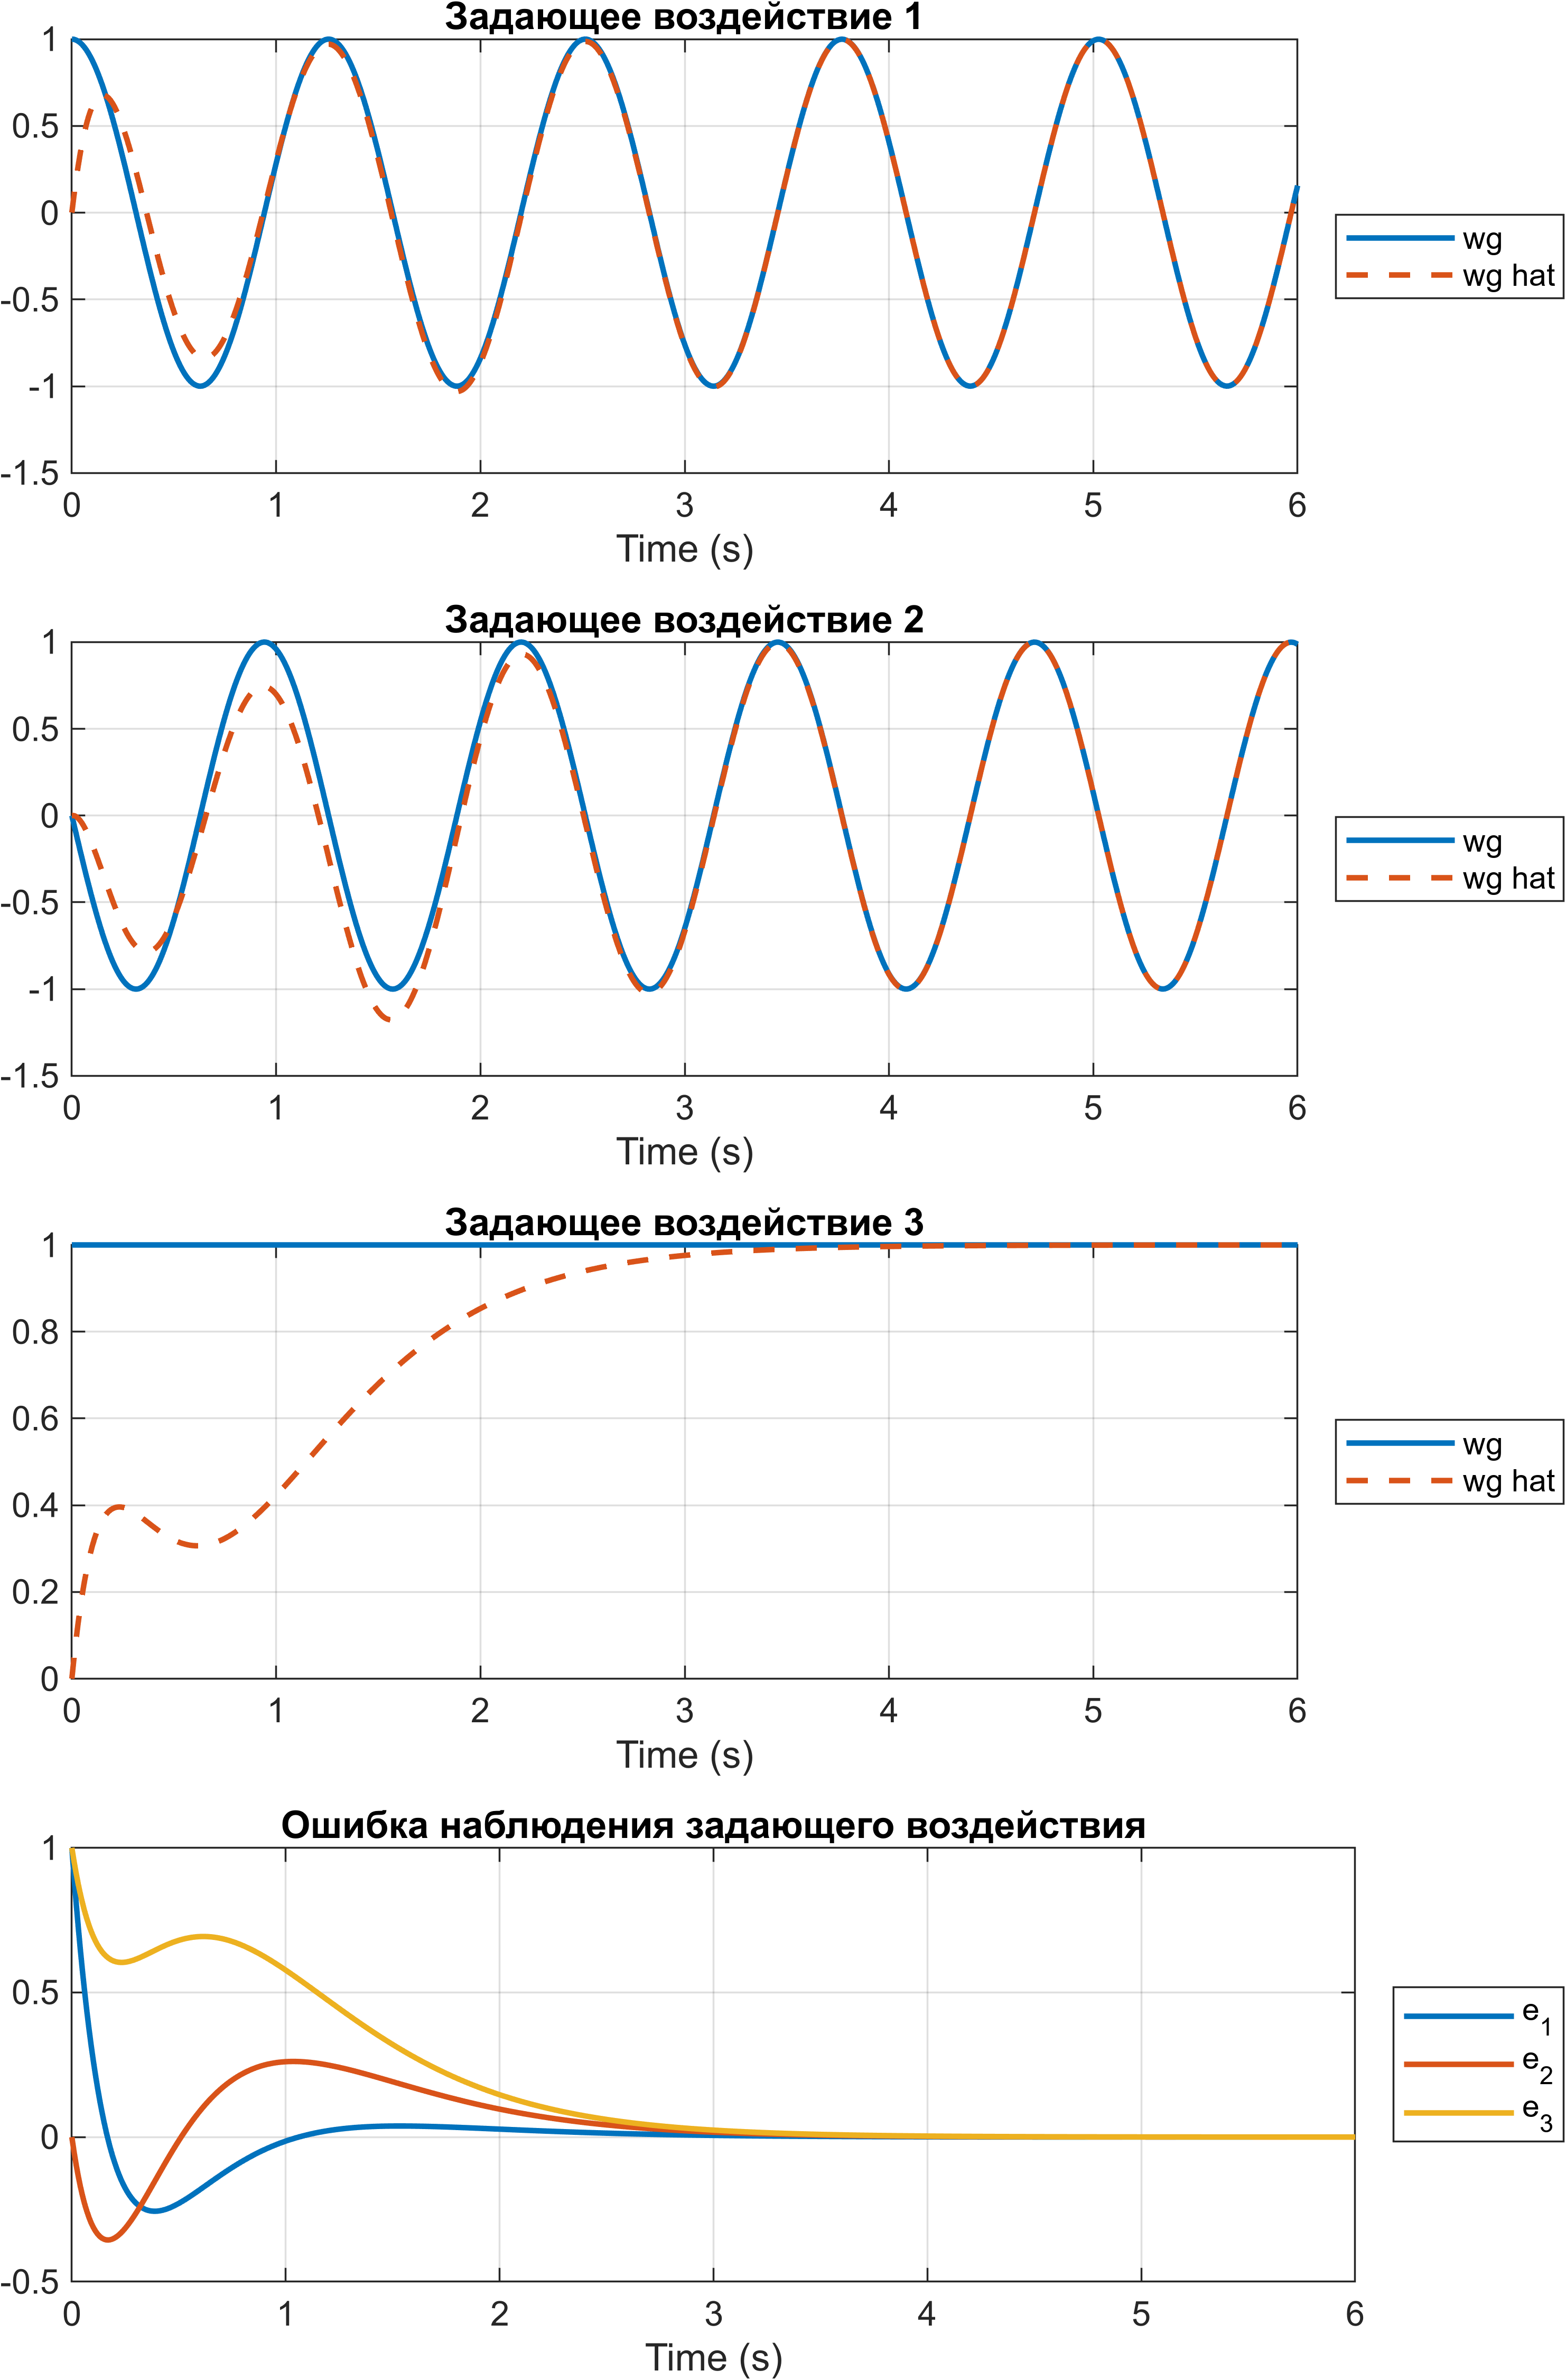
\includegraphics[width=0.9\linewidth]{figs/23_sim.png}
    \caption{Графики задающего воздействия $w_g(t)$, его оценки $\hat w_g(t)$ 
    и ошибки наблюдения $w_g(t)-\hat w_g(t)$}
    \label{fig:23}
\end{figure}

\subsection{Выводы}

В результате моделирования показано, что регулятор \eqref{eq:reg2}, 
основанный на наблюдателях, обеспечивает выполнение целевого условия 
\eqref{eq:goal1}. Ошибки наблюдения, такие как $w_f-\hat w_f$, $x-\hat x$, и $w_g-\hat w_g$, 
сходятся к нулю, что подтверждает корректность синтеза наблюдателей.
Сравнение с результатами Задания 1 показывает, что:
\begin{itemize}
    \item В обоих случаях целевое условие \eqref{eq:goal1} выполнено, и 
    выход системы $y(t)$ точно следует задающему воздействию $g(t)$.
    \item Использование наблюдателей в Задании 2 позволяет компенсировать 
    внешние возмущения и следить за задающим воздействием, даже если полное 
    состояния системы, внешнего и задающего воздействий недоступны для измерения.
\end{itemize}
Таким образом, регулятор \eqref{eq:reg2} с использованием наблюдателей 
является более универсальным решением, обеспечивающим выполнение целевого
условия \eqref{eq:goal1} в более реалистичных условиях.





\section{Слежение и компенсация: наблюдатели возмущения}

\subsection{Наблюдатель возмущения по состоянию}

\begin{figure}[H]
    \centering
    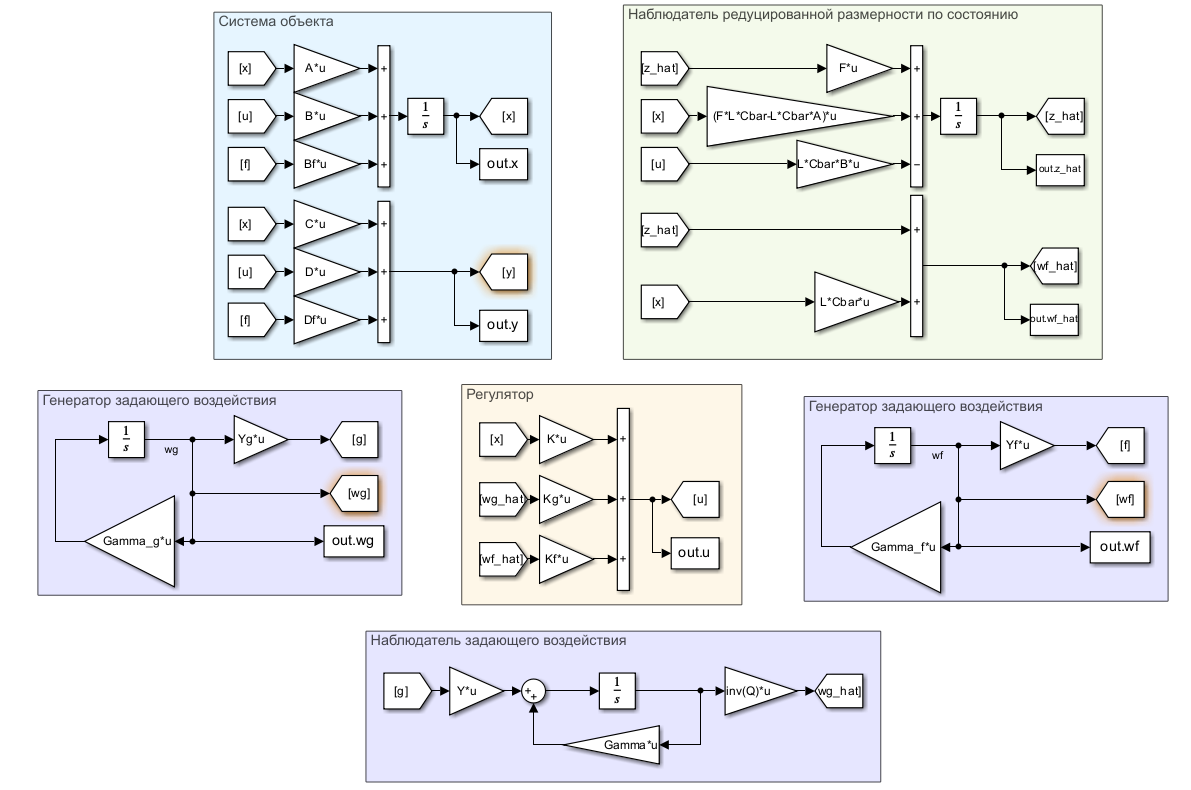
\includegraphics[width=\linewidth]{figs/31slx.png}
    \caption{Структурная схема для моделирования системы задания 3.1}
    \label{fig:30}
\end{figure}

Построим схему моделирования системы \eqref{eq:sys1}, замкнутой регулятором,
состоящим из наблюдателя задающего воздействия, наблюдателя возмущения редуцированной
размерности по состоянию и закона управления
\begin{equation}
    \label{eq:reg3}
    u=Kx+K_g\hat w_g+K_f\hat w_f,
\end{equation}
обеспечивающим выполнение целевого условия \eqref{eq:goal1}. Схему можно
увитдеть на \autoref{fig:30}.
Синтезируем наблюдатель возмущения:
\begin{equation*}
    \begin{cases}
        \hat{w_f}=\hat z+L\bar Cx,\\
        \dot{\hat z}=F\hat z+(FL\bar C-L\bar CA)x-L\bar CBu,
    \end{cases}
\end{equation*}
где $\bar C$ - матрица, удовлетворяющая уравнению $\bar CB_f=I$.
Пусть
\begin{equation*}
    \bar C=\begin{bmatrix}
        0	&-0.5000&	0\\
        0.5000	&-0.5000	&0
    \end{bmatrix}
\end{equation*}
Так же $F=\Gamma_f-LY_f$, матрица $L$ находится из решения уравнения Сильвестра
\begin{equation*}
    Q\Gamma-\Gamma_f^TQ=Y_f^TY,\quad L^T=-YQ^{-1}.
\end{equation*}
Подберем $\Gamma$ и $Y$, чтобы удовлетворялись условия существования решения
\begin{equation*}
    \Gamma=\begin{bmatrix}
        -1 & 0 & 0 & 0 \\
        0 & -2 & 0 & 0\\
        0 & 0 & -3 & 0\\
        0 & 0& 0& -4
    \end{bmatrix},\quad
    Y=\begin{bmatrix}
        1&1 & 1&1 \\ 1&1& 1&1
    \end{bmatrix},
\end{equation*}
тогда с помощью CVX получим
\begin{equation*}
    L=\begin{bmatrix}
        11.2500	&11.2500\\
        0.6250	&0.6250\\
        -3.7500	&-3.7500\\
        6.8750	&6.8750
    \end{bmatrix},\quad
    F=\begin{bmatrix}
        -10.0000	&-11.5000	&-11.7500&	3.0000\\
        -13.5000	&-20.7500	&-8.8750&	14.5000\\
        9.0000&	12.5000&	6.2500	&-5.0000\\
        -16.5000	&-23.2500	&-14.6250&	14.5000
    \end{bmatrix}.
\end{equation*}

Выполним компьютерное моделирование, графики управления, состояния, выхода и ошибки слежения 
можно увидеть на \autoref{fig:30_sim}, сравнительные графики внешнего возмущения,
его оценки и их разности на \autoref{fig:31_sim}.

\begin{figure}[H]
    \centering
    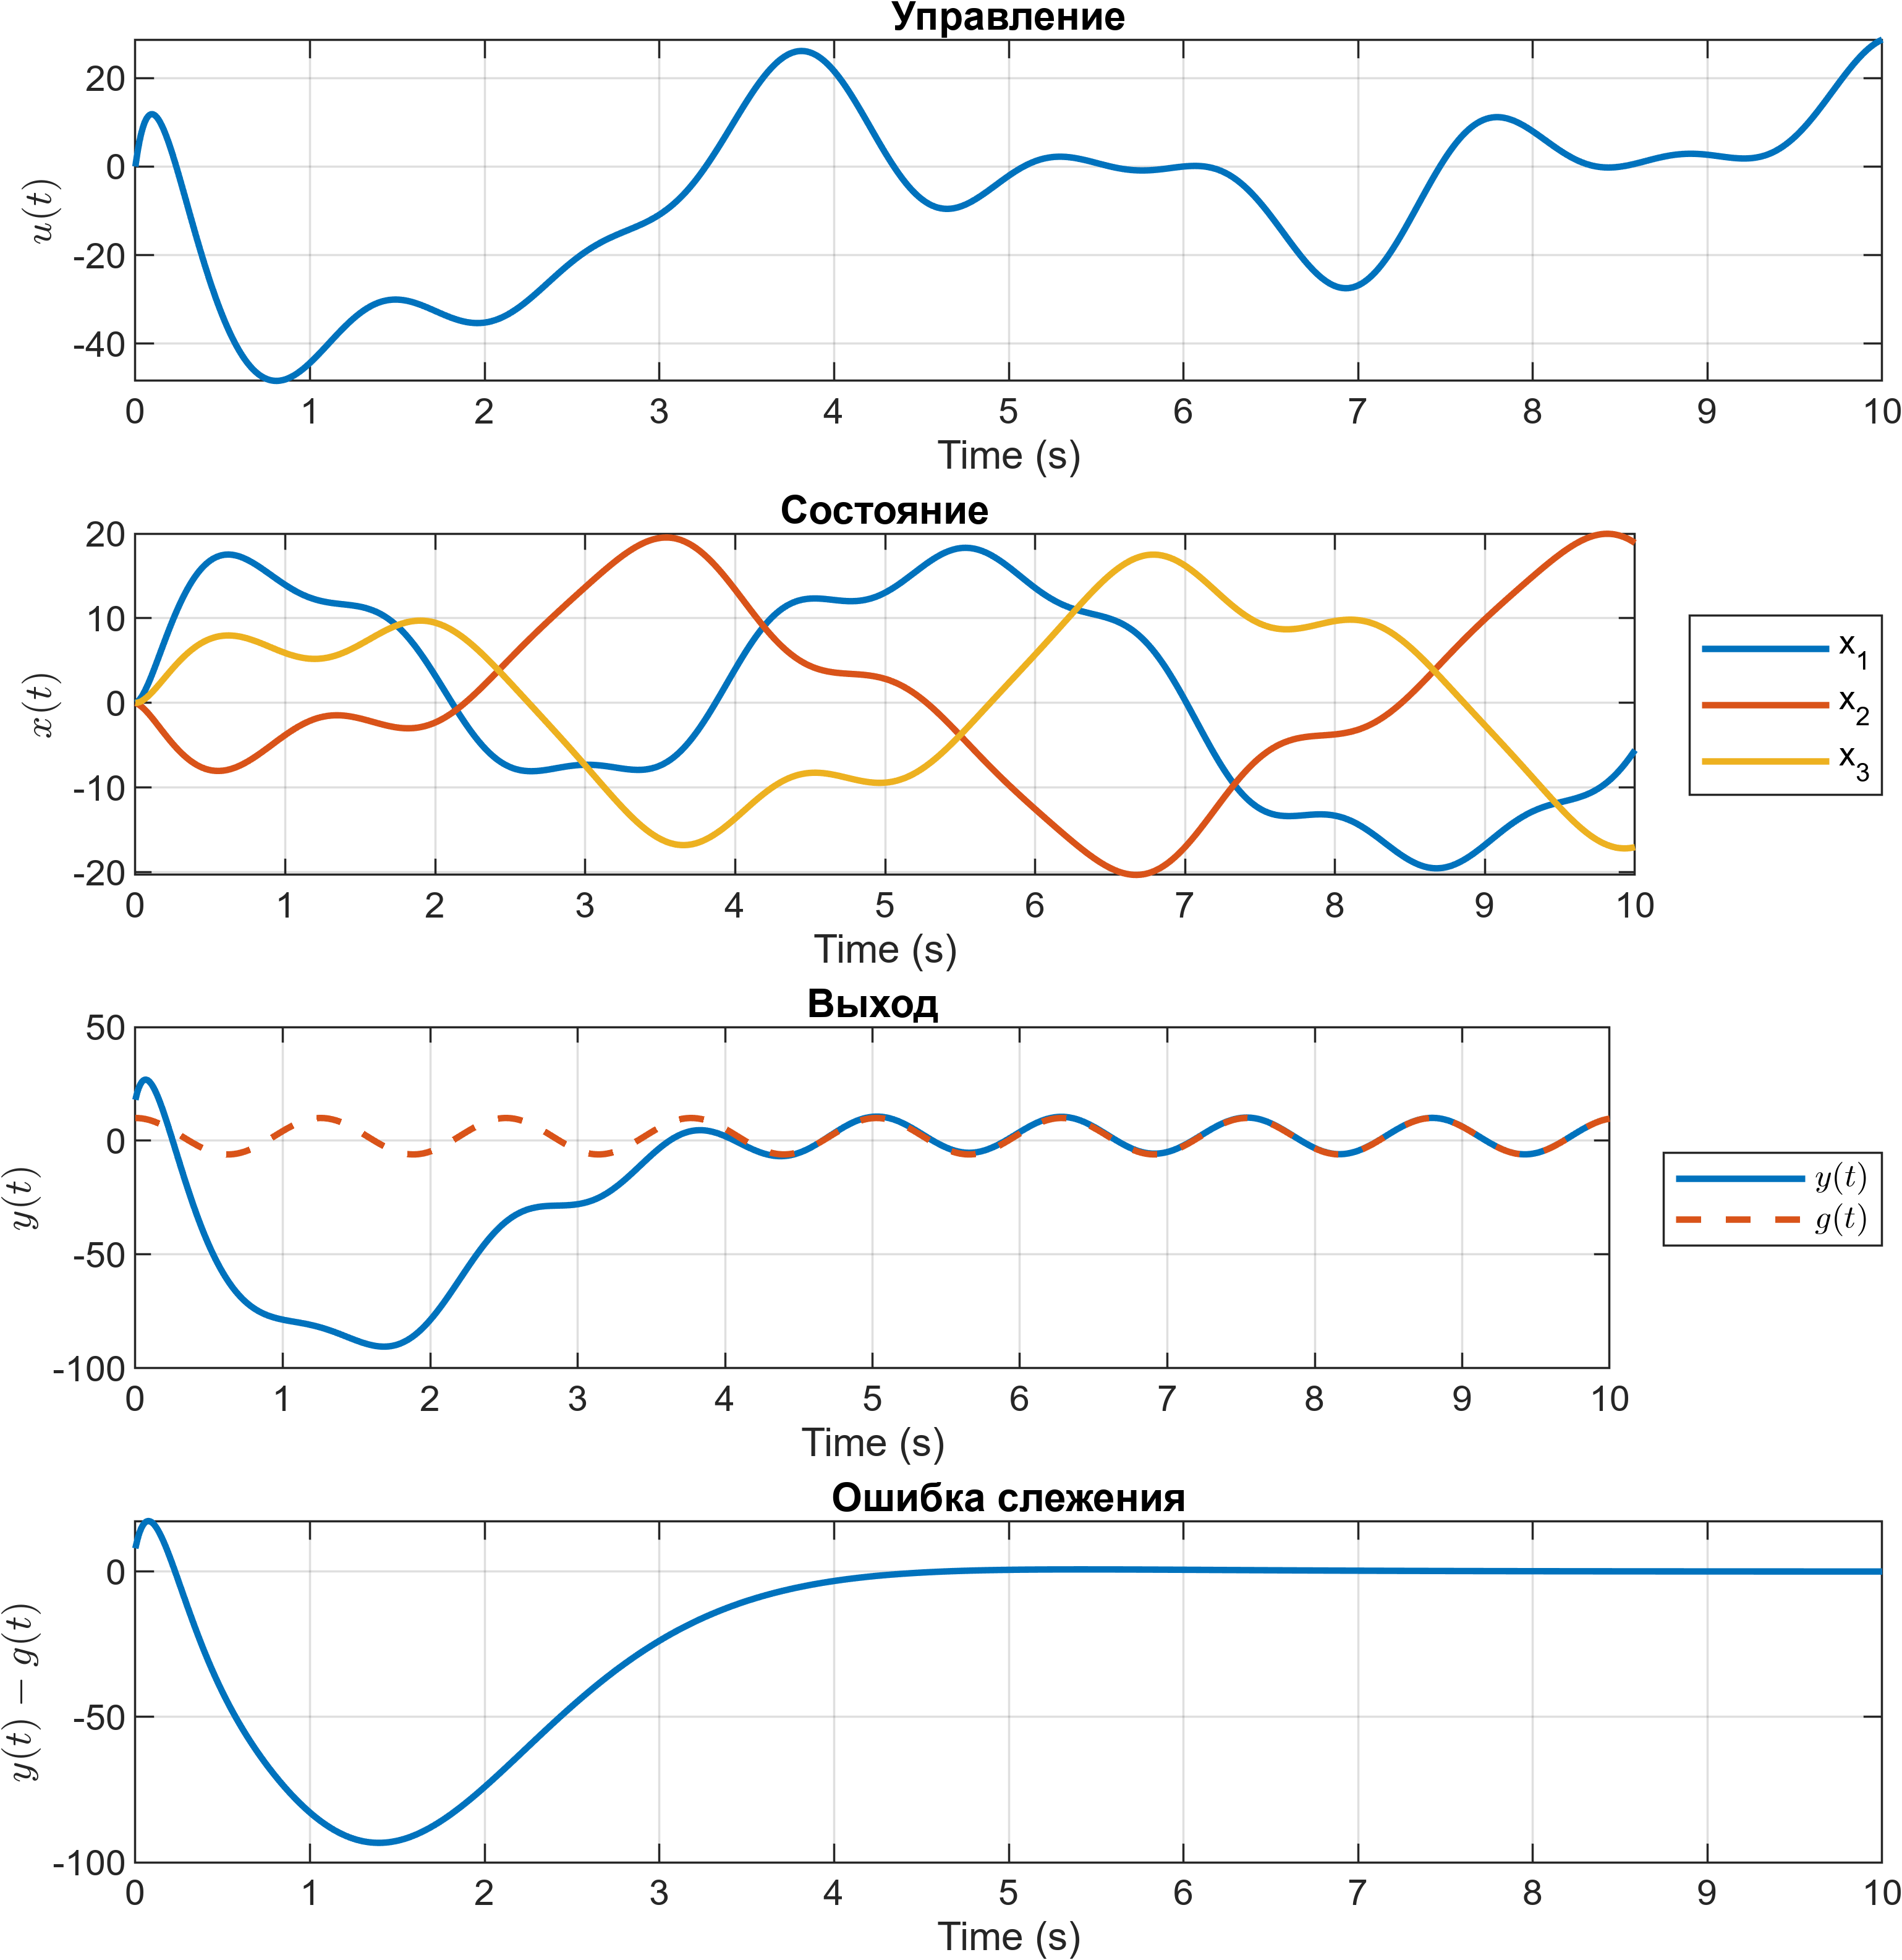
\includegraphics[width=\linewidth]{figs/30_sim.png}
    \caption{Графики управления, состояния, выхода и ошибки слежения}
    \label{fig:30_sim}
\end{figure}

\begin{figure}[H]
    \centering
    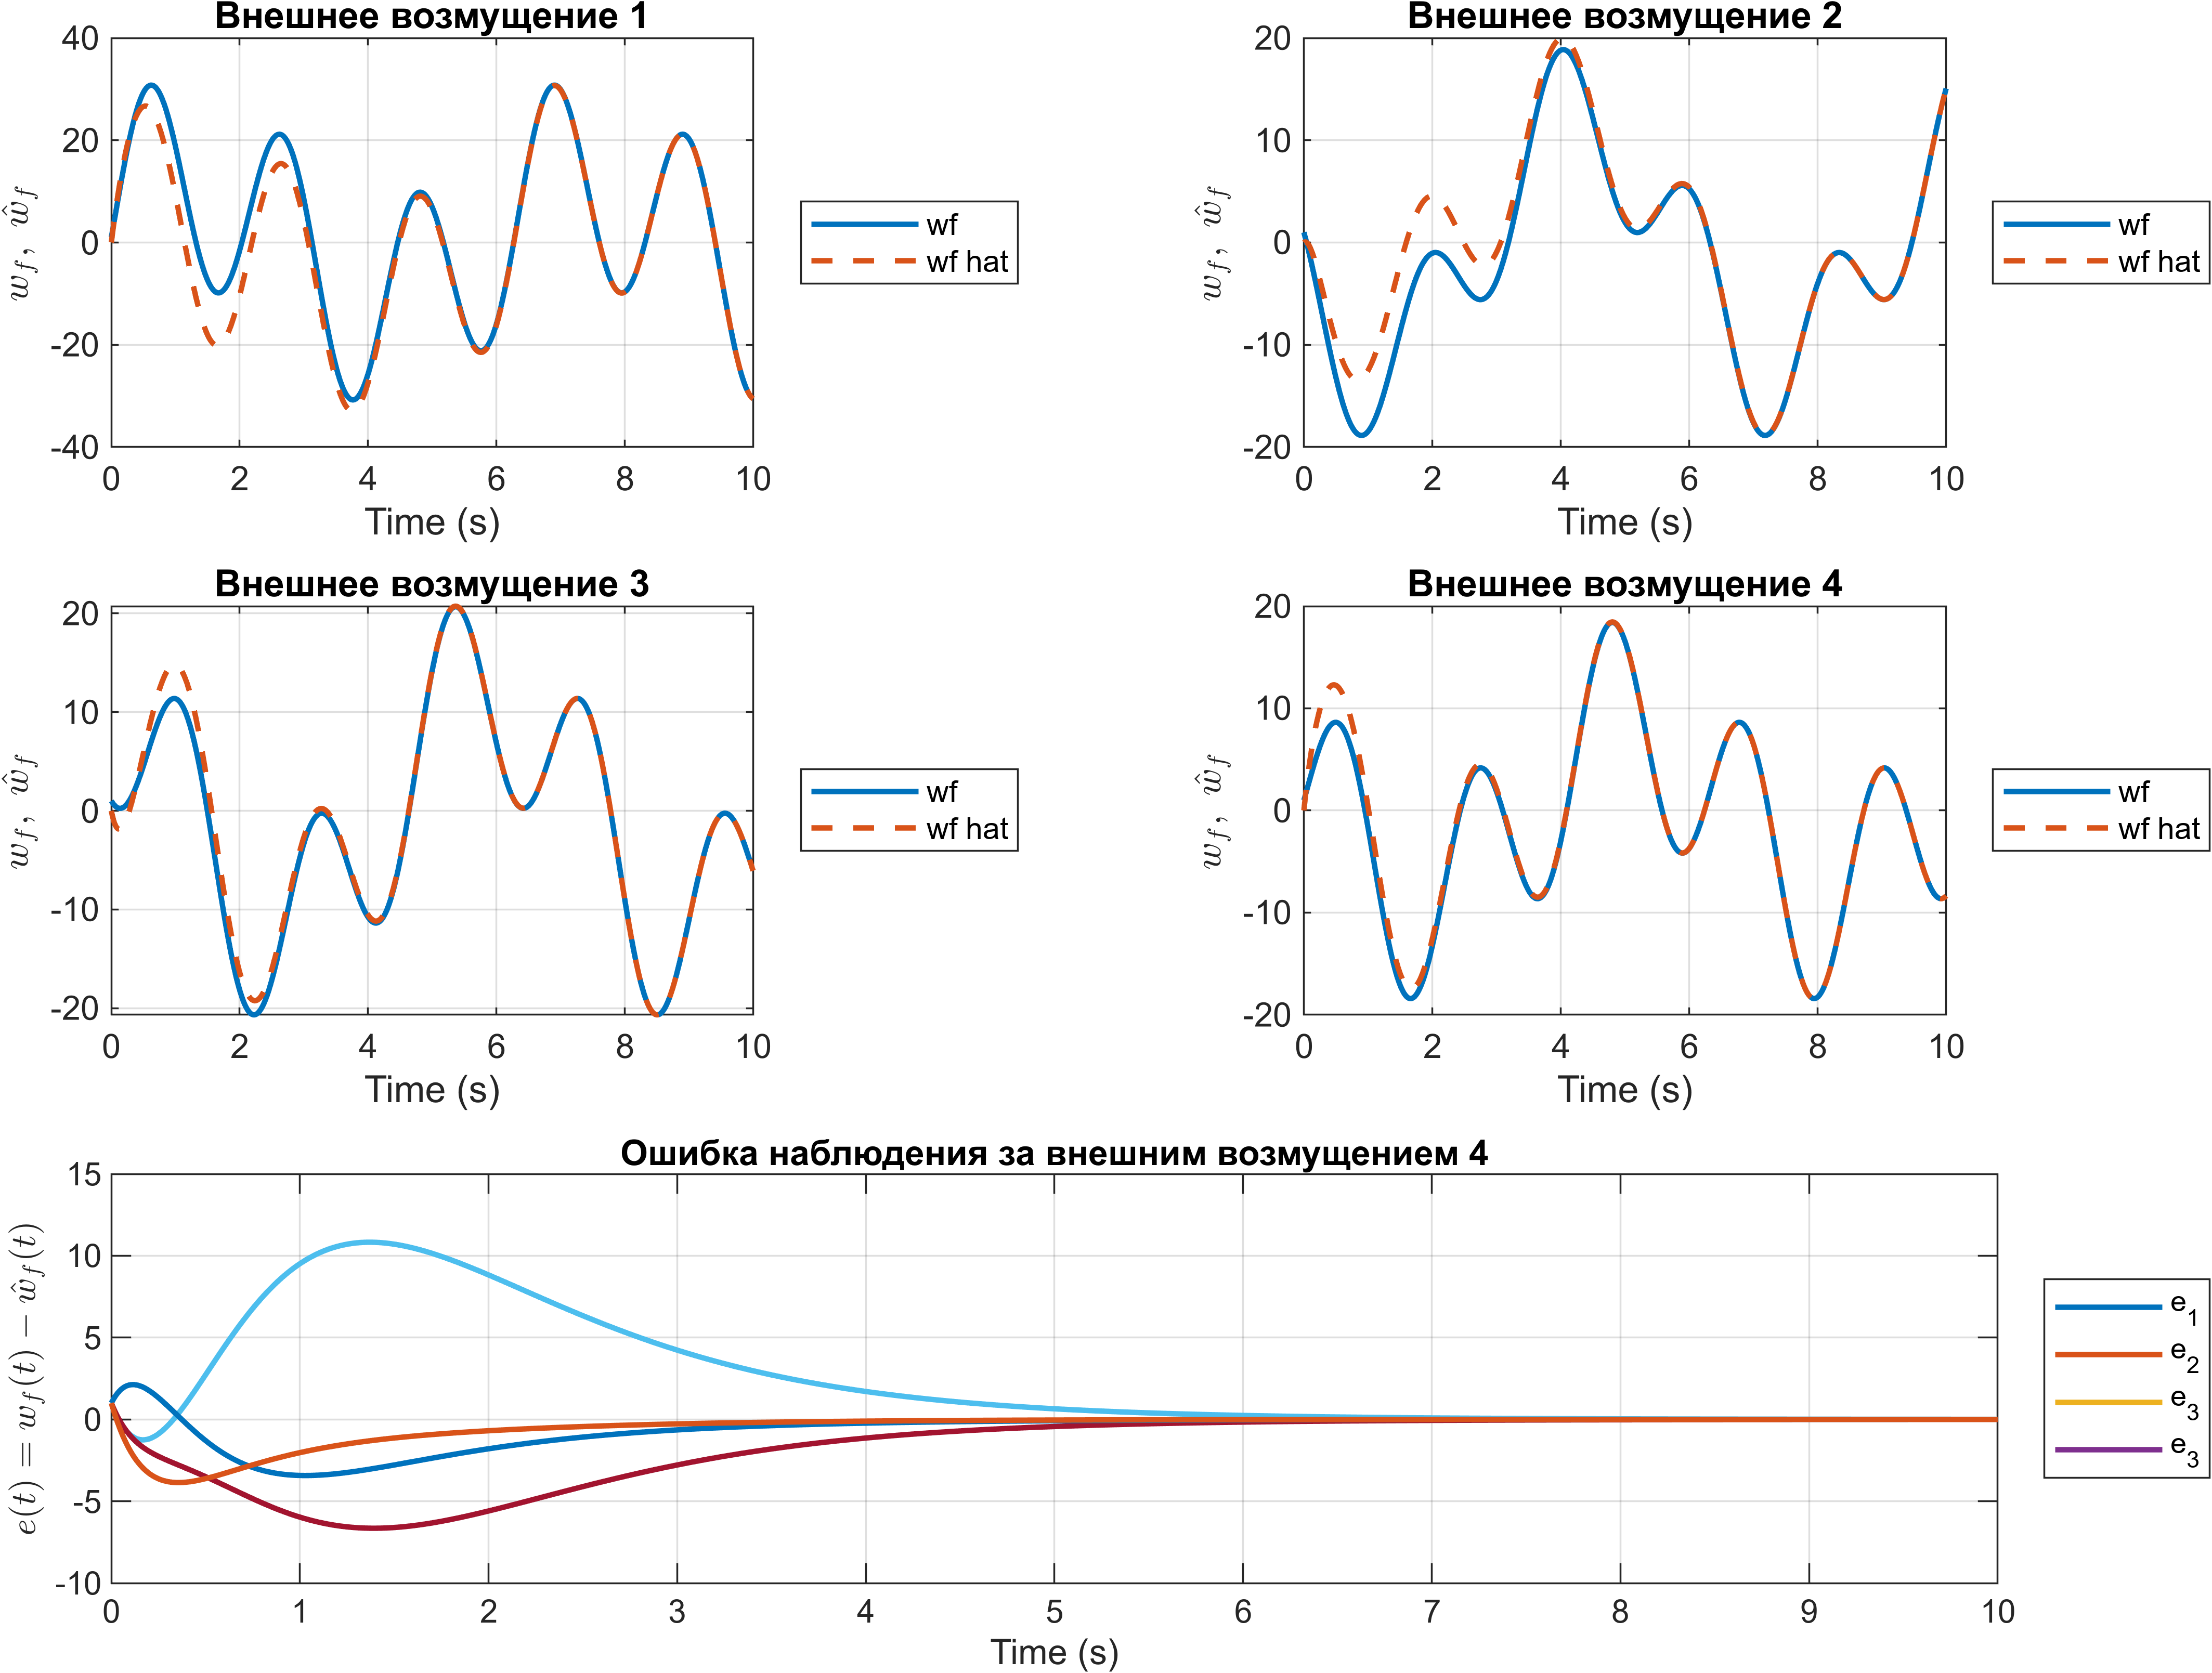
\includegraphics[width=\linewidth]{figs/31_sim.png}
    \caption{Графики  сравнительные графики внешнего возмущения,
    его оценки и их разности}
    \label{fig:31_sim}
\end{figure}



\subsection{Наблюдатель возмущения по выходу}

\begin{figure}[H]
    \centering
    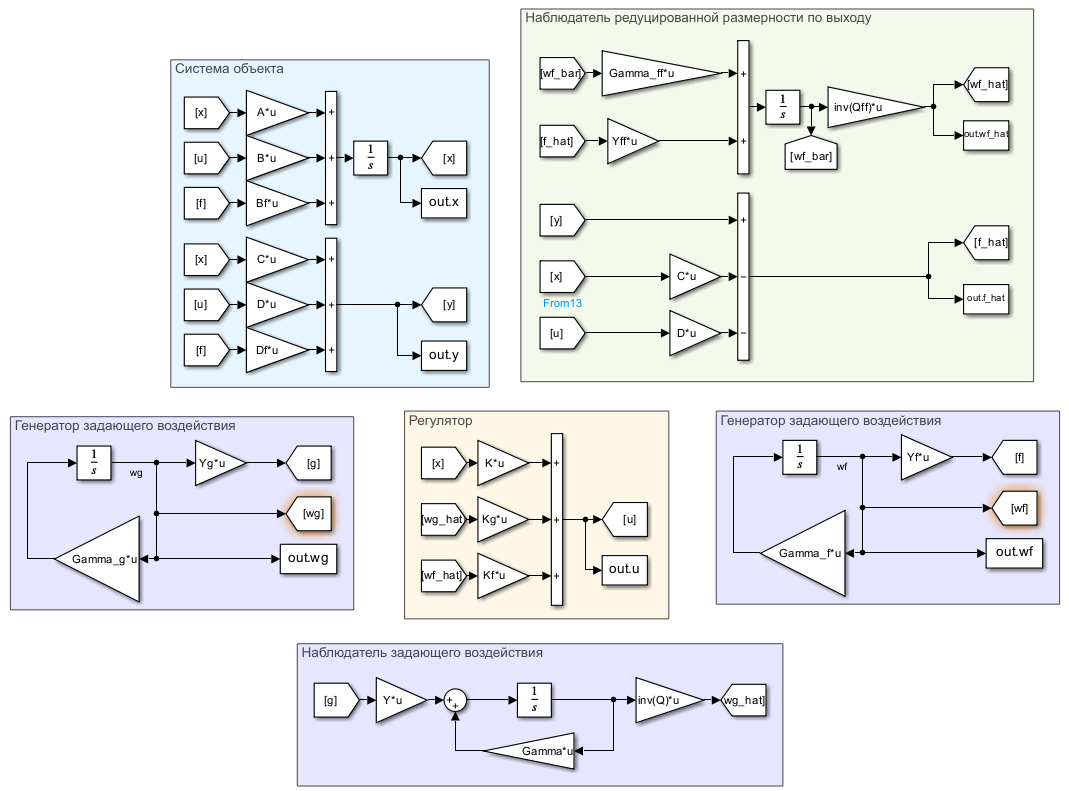
\includegraphics[width=\linewidth]{figs/32slx.png}
    \caption{Структурная схема для моделирования системы задания 3.2}
    \label{fig:31}
\end{figure}

Построим схему моделирования системы \eqref{eq:sys1}, замкнутой регулятором,
состоящим из наблюдателя задающего воздействия, наблюдателя возмущения редуцированной
размерности по выходу и закона управления \eqref{eq:reg3},
обеспечивающим выполнение целевого условия \eqref{eq:goal1}. Схему можно
увитдеть на \autoref{fig:31}.
Синтезируем наблюдатель возмущения:
\begin{equation*}
    \begin{cases}
        \hat f=y-Cx-Dx,\\
        \dot{\bar w}_f=\Gamma\bar w_f+Y\hat f,\\
        \hat w_f=Q^{-1}\bar w_f,
    \end{cases}
\end{equation*}
где матрица $Q$ находится из решения уравнения Сильвестра
\begin{equation*}
    Q\Gamma_f-\Gamma Q=YD_fY_f.
\end{equation*}
Подберем $\Gamma$ и $Y$, чтобы удовлетворялись условия существования решения
\begin{equation*}
    \Gamma=\begin{bmatrix}
        -1 & 0 & 0 & 0 \\
        0 & -2 & 0 & 0\\
        0 & 0 & -3 & 0\\
        0 & 0& 0& -4
    \end{bmatrix},\quad
    Y=\begin{bmatrix}
        1 \\ 1\\1\\ 1
    \end{bmatrix},
\end{equation*}
тогда с помощью CVX получим
\begin{equation*}
    Q=\begin{bmatrix}
            9.9000 & 15.4000 & 8.0000 & -12.0000 \\
            4.8923 & 7.8462 & 4.1538 & -5.7077 \\
            2.9000 & 4.7333 & 2.5333 & -3.2667 \\
            2.0047 & 3.3082 & 1.7741 & -2.1953
        \end{bmatrix}
\end{equation*}

Выполним компьютерное моделирование, графики управления, состояния, выхода и ошибки слежения 
можно увидеть на \autoref{fig:32_sim}, сравнительные графики внешнего возмущения,
его оценки и их разности на \autoref{fig:33_sim}.

\begin{figure}[H]
    \centering
    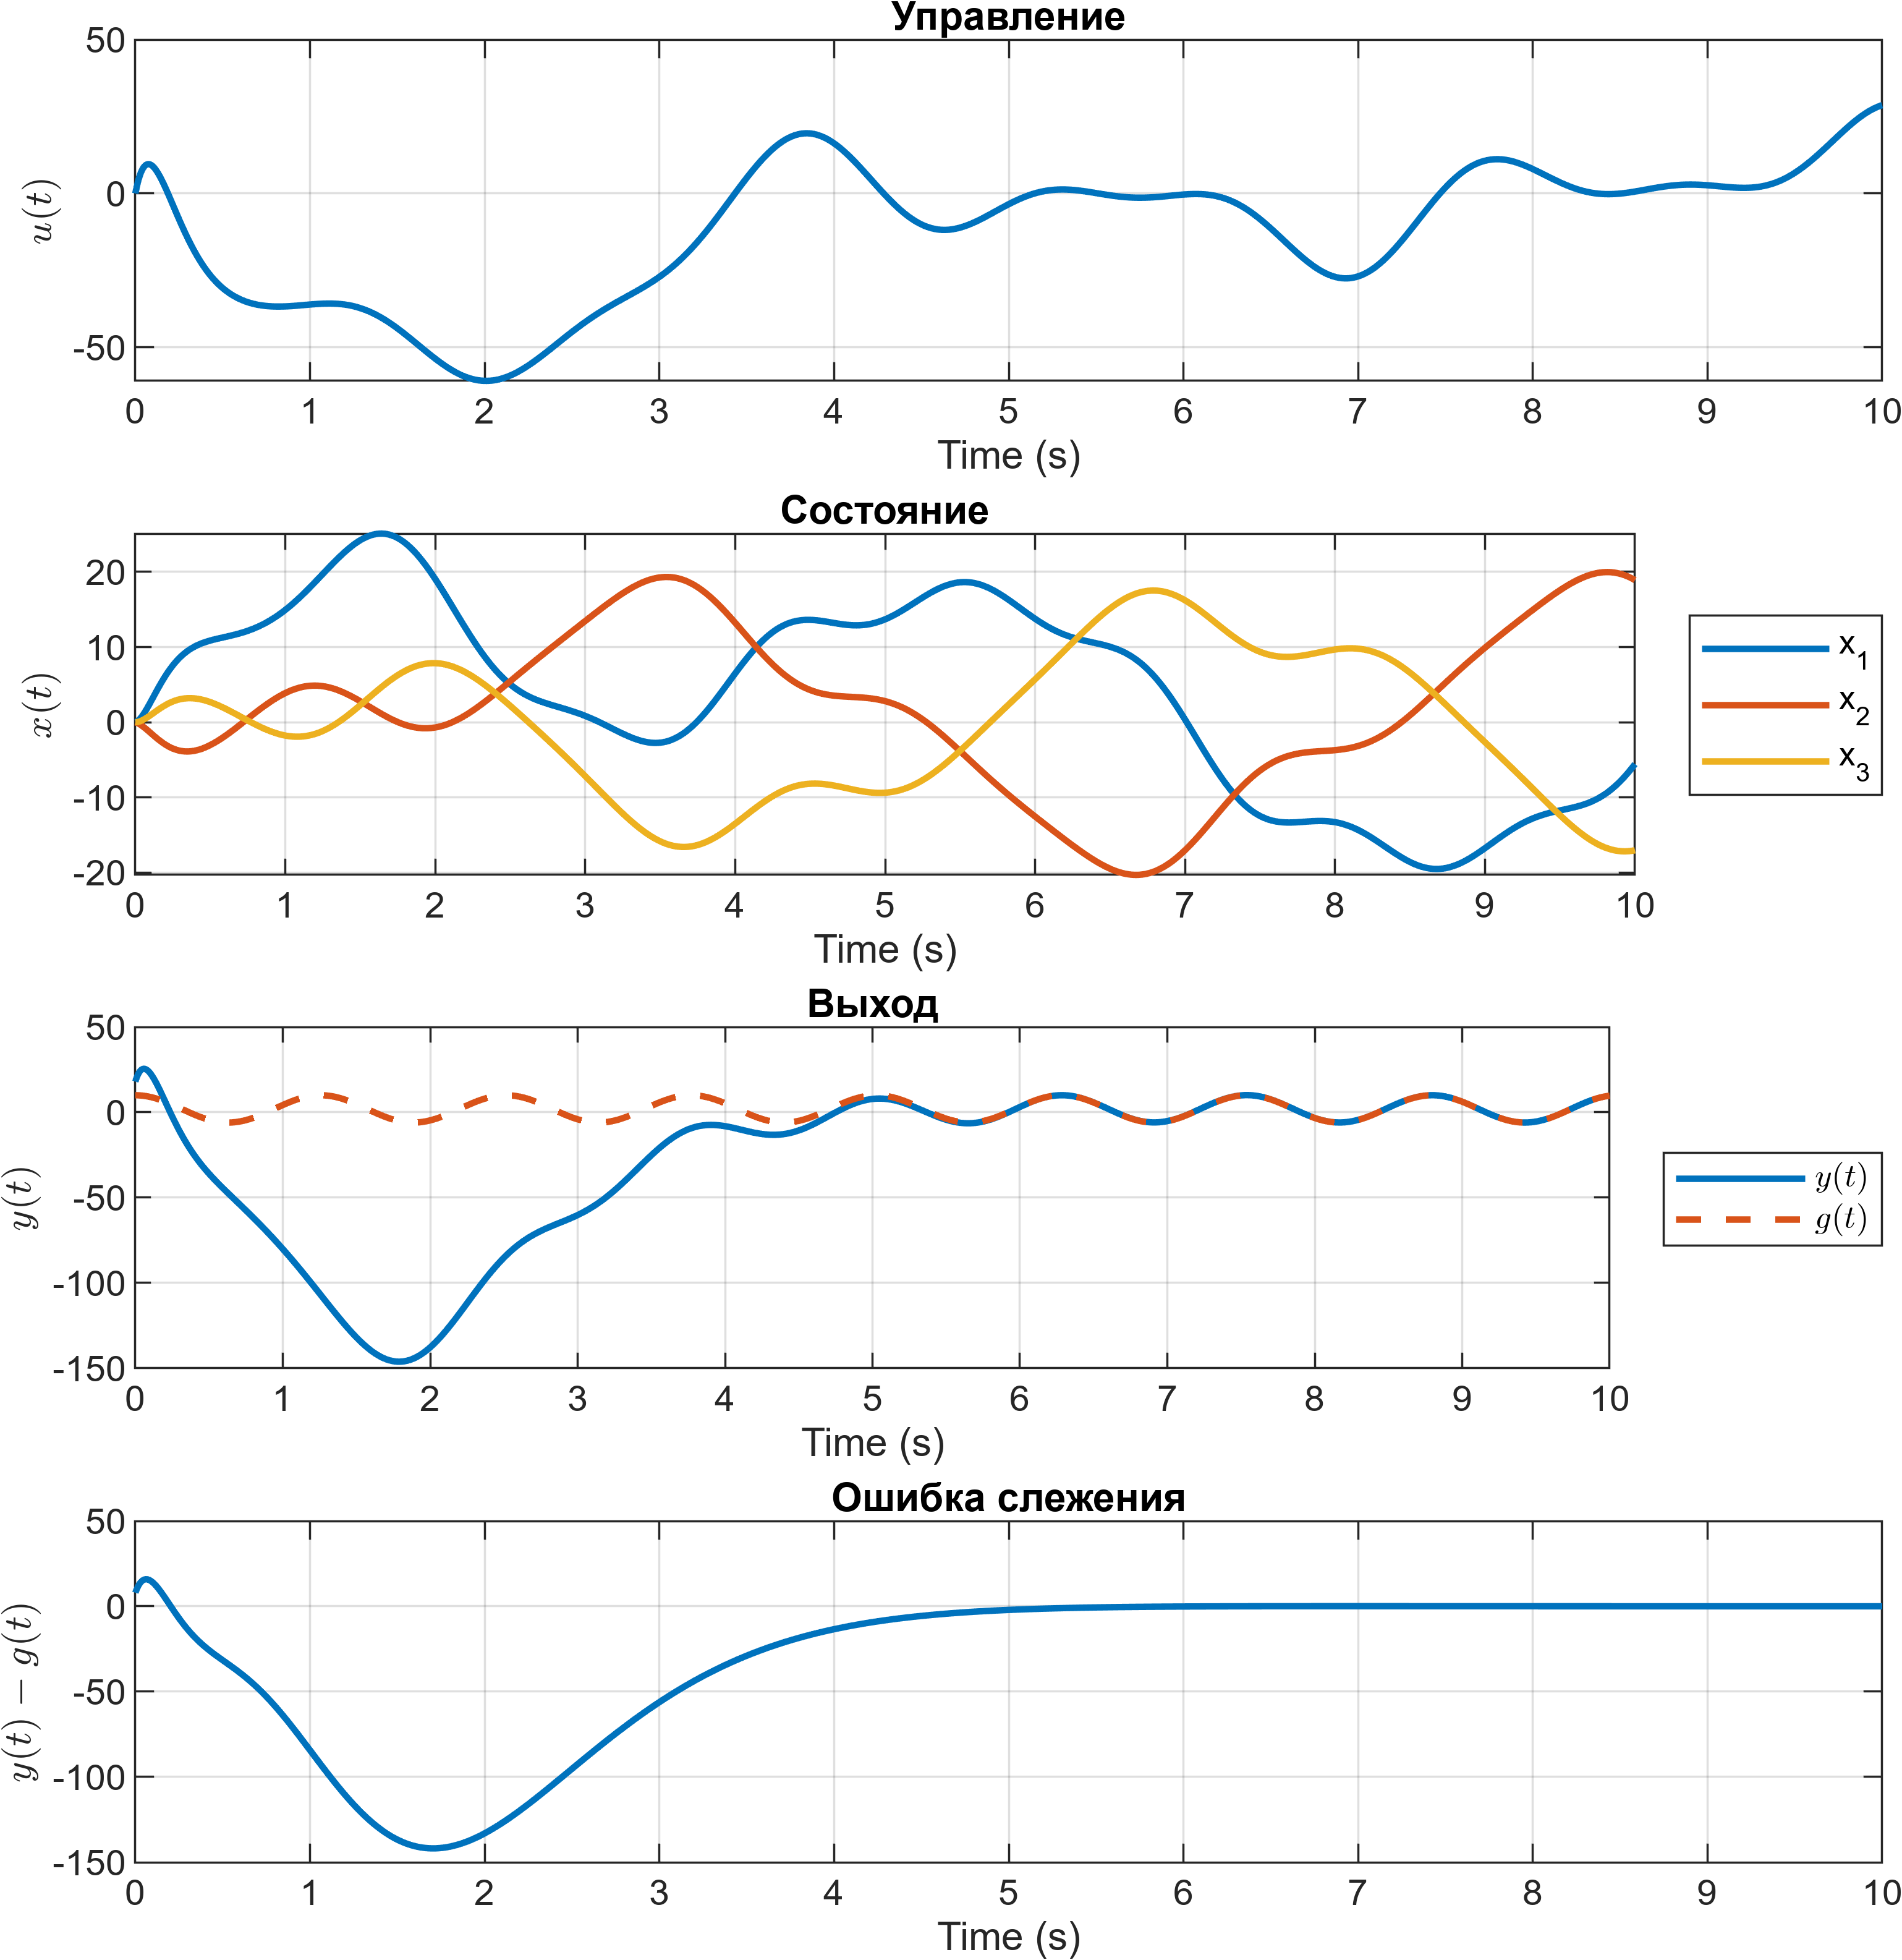
\includegraphics[width=\linewidth]{figs/32_sim.png}
    \caption{Графики управления, состояния, выхода и ошибки слежения}
    \label{fig:32_sim}
\end{figure}

\begin{figure}[H]
    \centering
    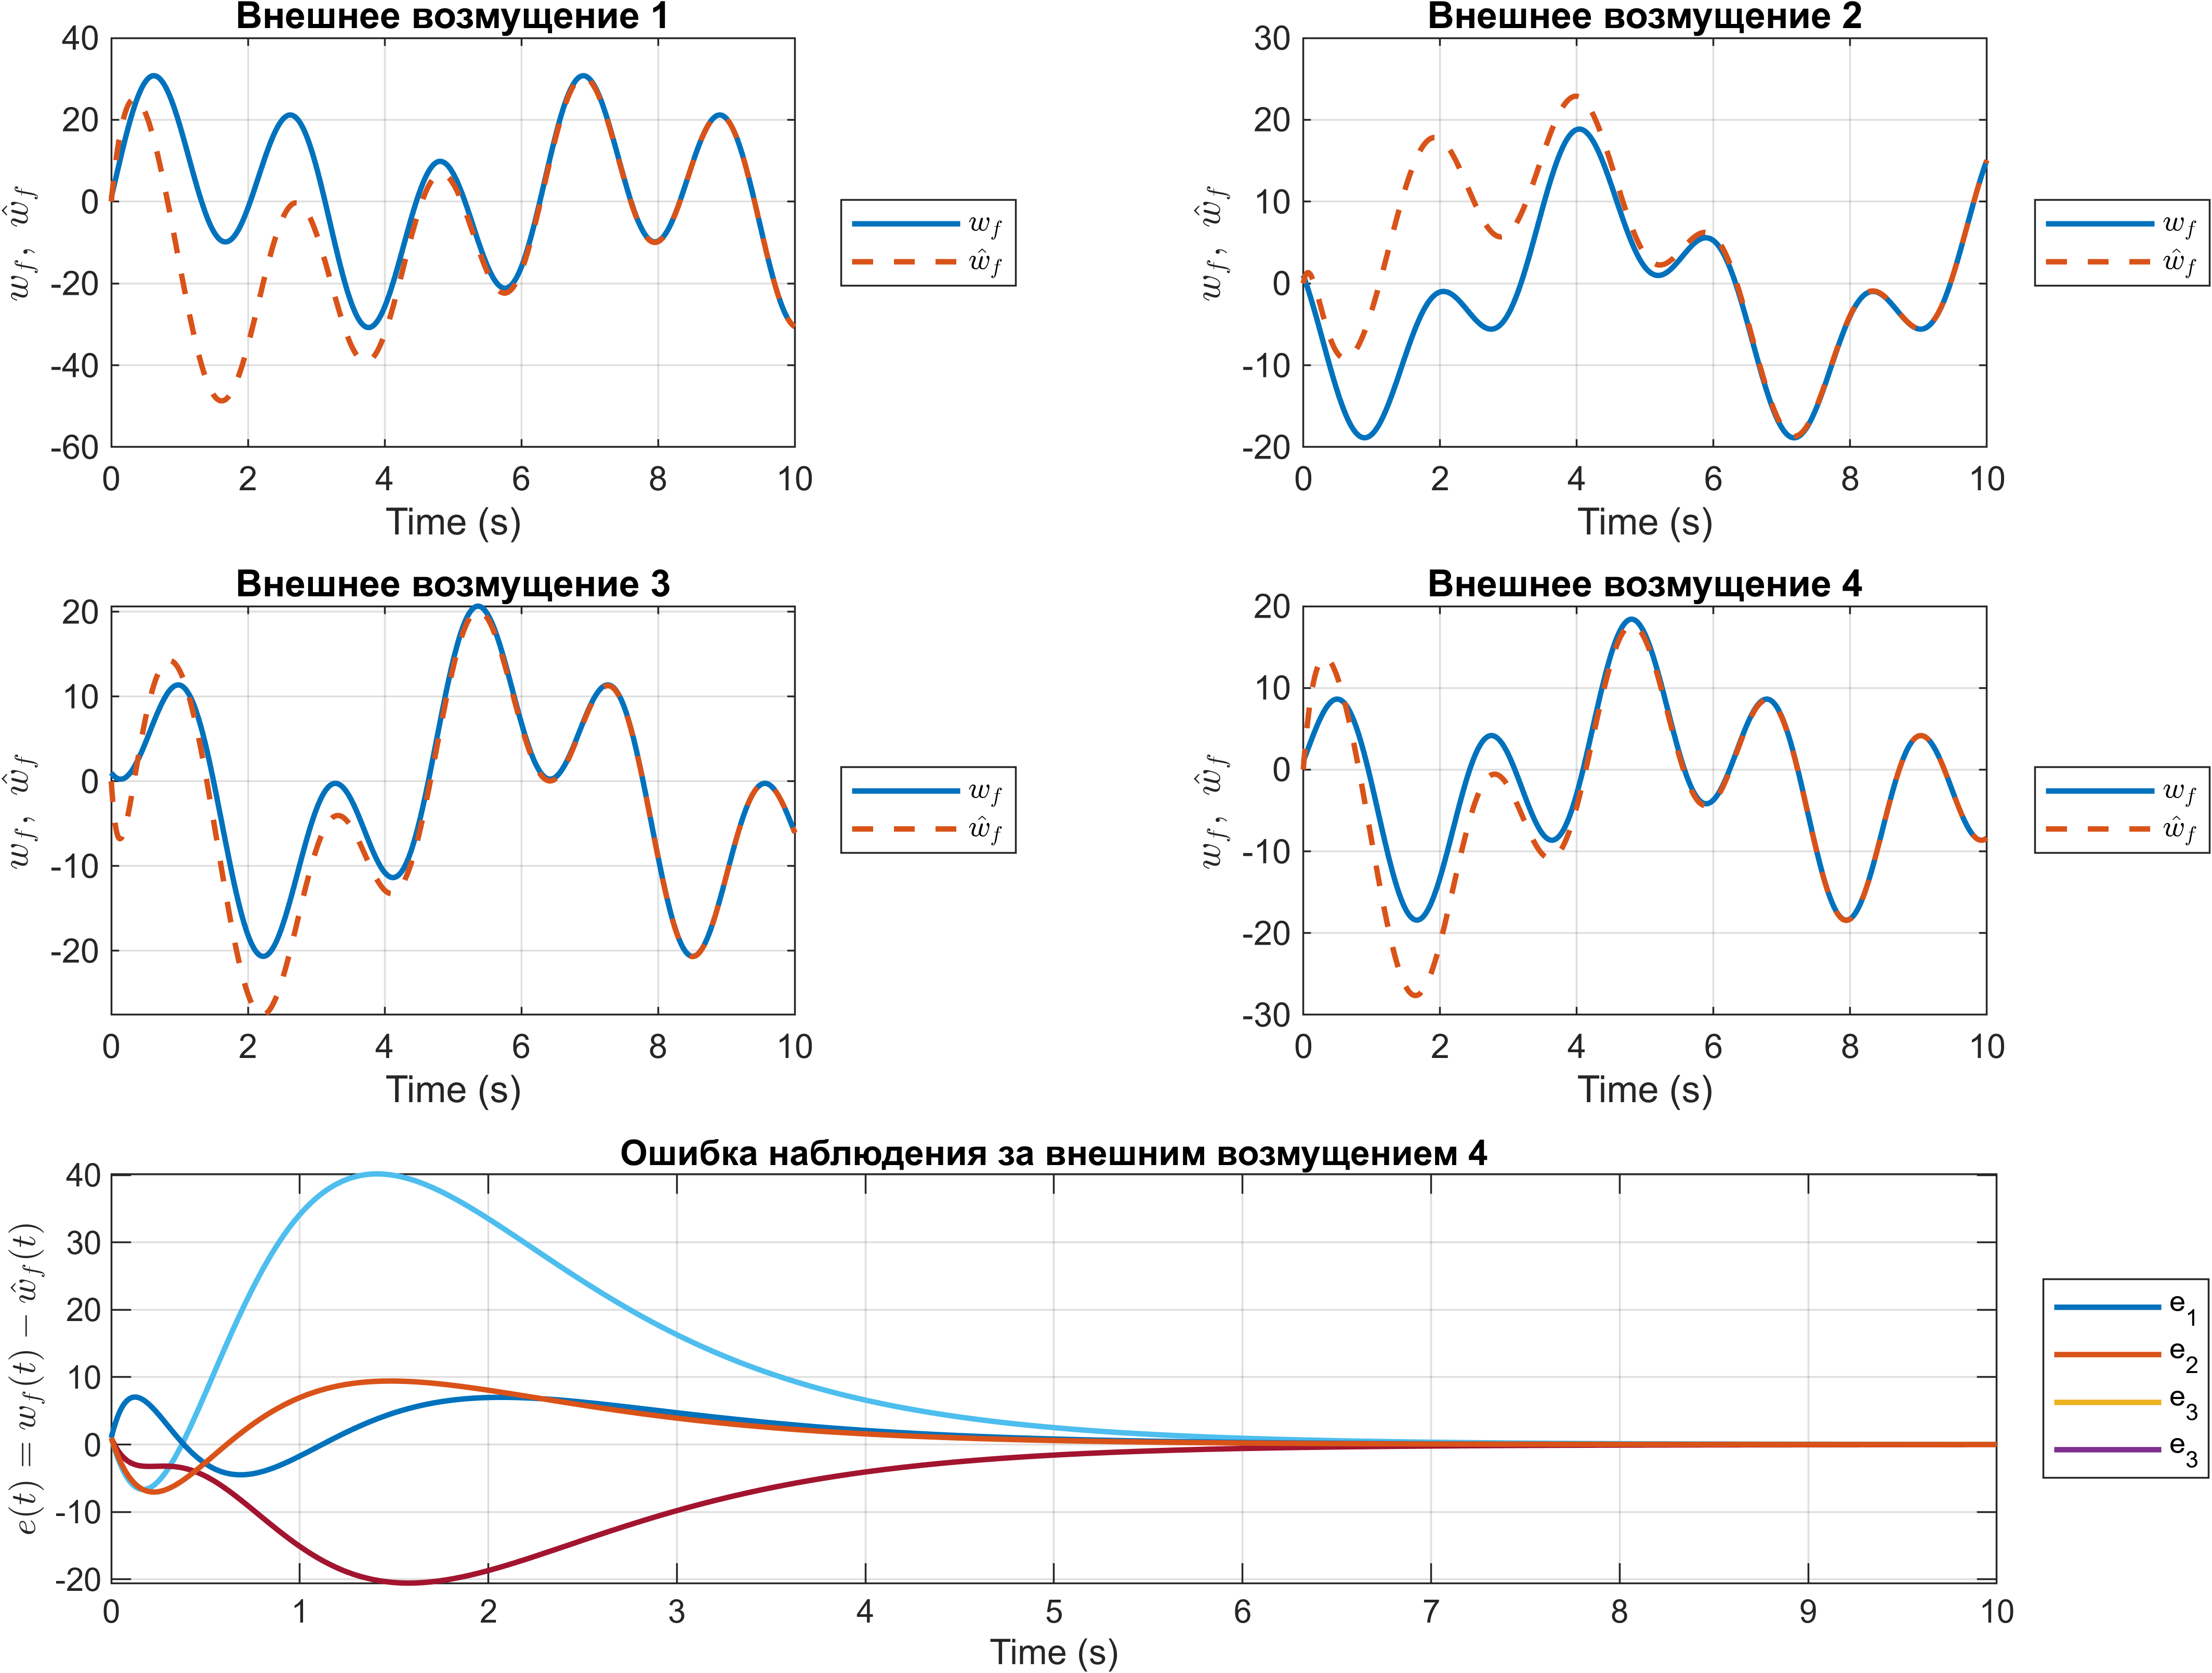
\includegraphics[width=\linewidth]{figs/33_sim.png}
    \caption{Графики  сравнительные графики внешнего возмущения,
    его оценки и их разности}
    \label{fig:33_sim}
\end{figure}



\subsection{Выводы}

Поведения редуцированных наблюдателей очень похоже, но редуцированный наблюдатель по 
состоянию показывает лучшие результаты:
\begin{enumerate}
    \item Ошибка слежения более гладкая
    \item Потребовалось "меньше" управления
    \item Выход имеем меньшую амплитуду
    \item Выход быстрее сошелся, но не намного, около полусекунды быстрее
\end{enumerate}
Таким образом, регулятор с редуцированным наблюдателем по состоянию показывает лучшие характеристики,
в сравнении с регулятором с редуцированным наблюдателем по выходу.

Сравнивая с регулятором из второго задания с наблюдателем расширенной размерности,
системы с редуцированным наблюдателем требовали гораздо меньше управления,
но и сходятся эти системы где-то в три раза медленнее.
Но использование редуцированных наблюдателей снижает вычислительную 
сложность и ресурсоемкость реализации регулятора.


\section{Заключение}

В данной лабораторной работе были исследованы различные подходы к проектированию 
наблюдателей и регуляторов. Проведённый анализ показал, что редуцированные наблюдатели 
по состоянию обеспечивают лучшие характеристики слежения и управления, снижая 
вычислительную сложность. Однако, их использование приводит к более медленной 
сходимости системы по сравнению с наблюдателями расширенной размерности. Таким образом, 
выбор подхода зависит от требований к быстродействию и ресурсам системы.
